% Options for packages loaded elsewhere
\PassOptionsToPackage{unicode}{hyperref}
\PassOptionsToPackage{hyphens}{url}
%
\documentclass[
  english,
  man,floatsintext]{apa6}
\usepackage{amsmath,amssymb}
\usepackage{lmodern}
\usepackage{ifxetex,ifluatex}
\ifnum 0\ifxetex 1\fi\ifluatex 1\fi=0 % if pdftex
  \usepackage[T1]{fontenc}
  \usepackage[utf8]{inputenc}
  \usepackage{textcomp} % provide euro and other symbols
\else % if luatex or xetex
  \usepackage{unicode-math}
  \defaultfontfeatures{Scale=MatchLowercase}
  \defaultfontfeatures[\rmfamily]{Ligatures=TeX,Scale=1}
\fi
% Use upquote if available, for straight quotes in verbatim environments
\IfFileExists{upquote.sty}{\usepackage{upquote}}{}
\IfFileExists{microtype.sty}{% use microtype if available
  \usepackage[]{microtype}
  \UseMicrotypeSet[protrusion]{basicmath} % disable protrusion for tt fonts
}{}
\makeatletter
\@ifundefined{KOMAClassName}{% if non-KOMA class
  \IfFileExists{parskip.sty}{%
    \usepackage{parskip}
  }{% else
    \setlength{\parindent}{0pt}
    \setlength{\parskip}{6pt plus 2pt minus 1pt}}
}{% if KOMA class
  \KOMAoptions{parskip=half}}
\makeatother
\usepackage{xcolor}
\IfFileExists{xurl.sty}{\usepackage{xurl}}{} % add URL line breaks if available
\IfFileExists{bookmark.sty}{\usepackage{bookmark}}{\usepackage{hyperref}}
\hypersetup{
  pdftitle={Cognitive Music Listening Space: A Multivariate Approach},
  pdfauthor={Brendon Mizener1, Mathilde Vandenberghe2, Hervé Abdi1, \& Sylvie Chollet2},
  pdflang={en-EN},
  pdfkeywords={Music, Perception, Cognition, Multivariate Analyses},
  hidelinks,
  pdfcreator={LaTeX via pandoc}}
\urlstyle{same} % disable monospaced font for URLs
\usepackage{graphicx}
\makeatletter
\def\maxwidth{\ifdim\Gin@nat@width>\linewidth\linewidth\else\Gin@nat@width\fi}
\def\maxheight{\ifdim\Gin@nat@height>\textheight\textheight\else\Gin@nat@height\fi}
\makeatother
% Scale images if necessary, so that they will not overflow the page
% margins by default, and it is still possible to overwrite the defaults
% using explicit options in \includegraphics[width, height, ...]{}
\setkeys{Gin}{width=\maxwidth,height=\maxheight,keepaspectratio}
% Set default figure placement to htbp
\makeatletter
\def\fps@figure{htbp}
\makeatother
\setlength{\emergencystretch}{3em} % prevent overfull lines
\providecommand{\tightlist}{%
  \setlength{\itemsep}{0pt}\setlength{\parskip}{0pt}}
\setcounter{secnumdepth}{-\maxdimen} % remove section numbering
% Make \paragraph and \subparagraph free-standing
\ifx\paragraph\undefined\else
  \let\oldparagraph\paragraph
  \renewcommand{\paragraph}[1]{\oldparagraph{#1}\mbox{}}
\fi
\ifx\subparagraph\undefined\else
  \let\oldsubparagraph\subparagraph
  \renewcommand{\subparagraph}[1]{\oldsubparagraph{#1}\mbox{}}
\fi
% Manuscript styling
\usepackage{upgreek}
\captionsetup{font=singlespacing,justification=justified}

% Table formatting
\usepackage{longtable}
\usepackage{lscape}
% \usepackage[counterclockwise]{rotating}   % Landscape page setup for large tables
\usepackage{multirow}		% Table styling
\usepackage{tabularx}		% Control Column width
\usepackage[flushleft]{threeparttable}	% Allows for three part tables with a specified notes section
\usepackage{threeparttablex}            % Lets threeparttable work with longtable

% Create new environments so endfloat can handle them
% \newenvironment{ltable}
%   {\begin{landscape}\begin{center}\begin{threeparttable}}
%   {\end{threeparttable}\end{center}\end{landscape}}
\newenvironment{lltable}{\begin{landscape}\begin{center}\begin{ThreePartTable}}{\end{ThreePartTable}\end{center}\end{landscape}}

% Enables adjusting longtable caption width to table width
% Solution found at http://golatex.de/longtable-mit-caption-so-breit-wie-die-tabelle-t15767.html
\makeatletter
\newcommand\LastLTentrywidth{1em}
\newlength\longtablewidth
\setlength{\longtablewidth}{1in}
\newcommand{\getlongtablewidth}{\begingroup \ifcsname LT@\roman{LT@tables}\endcsname \global\longtablewidth=0pt \renewcommand{\LT@entry}[2]{\global\advance\longtablewidth by ##2\relax\gdef\LastLTentrywidth{##2}}\@nameuse{LT@\roman{LT@tables}} \fi \endgroup}

% \setlength{\parindent}{0.5in}
% \setlength{\parskip}{0pt plus 0pt minus 0pt}

% \usepackage{etoolbox}
\makeatletter
\patchcmd{\HyOrg@maketitle}
  {\section{\normalfont\normalsize\abstractname}}
  {\section*{\normalfont\normalsize\abstractname}}
  {}{\typeout{Failed to patch abstract.}}
\patchcmd{\HyOrg@maketitle}
  {\section{\protect\normalfont{\@title}}}
  {\section*{\protect\normalfont{\@title}}}
  {}{\typeout{Failed to patch title.}}
\makeatother
\shorttitle{Music Descriptor Space}
\keywords{Music, Perception, Cognition, Multivariate Analyses\newline\indent Word count: 5631}
\usepackage{csquotes}
\usepackage{caption}
\usepackage{subcaption}
\usepackage{wrapfig}
\ifxetex
  % Load polyglossia as late as possible: uses bidi with RTL langages (e.g. Hebrew, Arabic)
  \usepackage{polyglossia}
  \setmainlanguage[]{english}
\else
  \usepackage[main=english]{babel}
% get rid of language-specific shorthands (see #6817):
\let\LanguageShortHands\languageshorthands
\def\languageshorthands#1{}
\fi
\ifluatex
  \usepackage{selnolig}  % disable illegal ligatures
\fi
\newlength{\cslhangindent}
\setlength{\cslhangindent}{1.5em}
\newlength{\csllabelwidth}
\setlength{\csllabelwidth}{3em}
\newenvironment{CSLReferences}[2] % #1 hanging-ident, #2 entry spacing
 {% don't indent paragraphs
  \setlength{\parindent}{0pt}
  % turn on hanging indent if param 1 is 1
  \ifodd #1 \everypar{\setlength{\hangindent}{\cslhangindent}}\ignorespaces\fi
  % set entry spacing
  \ifnum #2 > 0
  \setlength{\parskip}{#2\baselineskip}
  \fi
 }%
 {}
\usepackage{calc}
\newcommand{\CSLBlock}[1]{#1\hfill\break}
\newcommand{\CSLLeftMargin}[1]{\parbox[t]{\csllabelwidth}{#1}}
\newcommand{\CSLRightInline}[1]{\parbox[t]{\linewidth - \csllabelwidth}{#1}\break}
\newcommand{\CSLIndent}[1]{\hspace{\cslhangindent}#1}

\title{Cognitive Music Listening Space: A Multivariate Approach}
\author{Brendon Mizener\textsuperscript{1}, Mathilde Vandenberghe\textsuperscript{2}, Hervé Abdi\textsuperscript{1}, \& Sylvie Chollet\textsuperscript{2}}
\date{}


\authornote{

Add complete departmental affiliations for each author here. Each new line herein must be indented, like this line.

Enter author note here.

The authors made the following contributions. Brendon Mizener: Stimuli creation, Survey design \& creation, Data collection \& processing, Statistical analyses, Writing - Original draft preparation; Mathilde Vandenberghe: Original concept, Survey design \& creation; Hervé Abdi: Writing - Review \& Editing, Statistical guidance; Sylvie Chollet: Original concept.

Correspondence concerning this article should be addressed to Brendon Mizener, 800 W. Campbell Rd., Richardson Tex. E-mail: \href{mailto:bmizener@utdallas.edu}{\nolinkurl{bmizener@utdallas.edu}}

}

\affiliation{\vspace{0.5cm}\textsuperscript{1} University of Texas at Dallas\\\textsuperscript{2} Junia, Univ. Artois, Université de Liège, Univ. Littoral Côte d'Opale, UMRT 1158 BioEcoAgro, F-62000 Arras, France}

\abstract{
French and American participants listened to new music stimuli and evaluated the stimuli using either adjectives or quantitative musical dimensions. Results were analyzed using Correspondence Analysis (CA), Hierarchical Cluster Analysis (HCA), Multiple Factor Analysis (MFA), and Partial Least Squares Correlation (PLSC). All except the HCA used Bootstrapping and Permutation testing for inferences. French and American listeners differed when they described the musical stimuli using adjectives, but not when using the quantitative dimensions. The present work serves as a case study in research methodology that allows for a balance between relaxing experimental control and maintaining statistical rigor.
}



\begin{document}
\maketitle

\begin{center}\rule{0.5\linewidth}{0.5pt}\end{center}

We have a data collection problem: World events over the last year have shown that we need to be able to collect good data outside of the lab. In the lab, because we control error sources, we measure, on relatively small sets of observations, a few well-defined, quantitative variables, analyzed using standard techniques such as analysis of variance (ANOVA). But, with the labs closed (remember COVID?), how can we collect good data? Away from the controlled environment of the lab, quantitative variables are hard to measure, but we can collect, on large sets of observations, qualitative variables that can only be analyzed by newer multivariate techniques. In the present paper, we present a case study illustrating this tradeoff.

Doesn't beer taste better in a bar? Or when you're listening to your favorite song? The present study was designed to quantify a music listening `space' that captures perceptual and cognitive dimensions for the sake of investigating cross-modal sensory mapping between beer drinking and music listening. It also addresses other questions: Are there differences in how people from different countries --- and by extension musical cultures --- perceive and describe music? And: What parallels exist between qualitative and quantitative descriptions of music?

For the present study, we have defined 1) perceptual dimensions as quantitative musical qualities, such as tempo, range, and meter and 2) cognitive dimensions as qualitative descriptions of music, such as `dark,' `warm,' and `round.' These cognitive/qualitative dimensions are similar to the commonly investigated affective or emotional dimensions, but do not specifically assess affective quality. We designed three experiments to quantify individual and combined spaces for these concepts, using separate surveys. The first experiment included highly trained musicians and featured a simple multiple choice survey about the perceptual dimensions; the second included participants with any level of music training performing a check-all-that-apply task (CATA, Katz \& Braly, 1933; Meyners \& Castura, 2014; Coombs et al., 1956); the third experiment incorporated both surveys in a single analysis.

To analyze our data, we selected a set of multivariate analyses that allowed us to visualize answers to each of our questions. The mental spaces revealed by the individual surveys were calculated and visualized using Correspondence Analysis (CA), a method similar to Principal Components Analysis (PCA) that analyzes qualitative data. We used Multidimensional Scaling (MDS), a distance analysis, to visualize the differences between participants and participant groups. To find parallels between the surveys, we used Partial Least Squares Correlation (PLSC), a method that analyzes two data tables with different sets of variables measured on the same observations. We used a Multiple Factor Analysis to evaluate how French and American participants' responses differed. Each of these analyses provide different visualizations and interpretations of the data, which are discussed in more detail below and in the discussion sections of each experiment.

\hypertarget{music-perception}{%
\subsection{Music Perception}\label{music-perception}}

Quantifying music perception is an interesting test case for this kind of data gathering and analytical paradigm. Most music or auditory perception studies have the inherent confound that small changes can affect listeners' perception, especially when the study involves timing, tuning, or sound localization. However, the experimental controls may be loosened slightly when investigating holistic music listening, because no single musical element is more important than the whole.

Quantitative and qualitative elements of music are theoretically distinct but practically inseparable (Bruner II, 1990). Listeners respond affectively to technical aspects of music using internal perceptual and cognitive schemata informed by their individual musical experiences and personality traits (Kopacz, 2005), and composers use various musical and compositional techniques to convey the emotions they want to express (Battcock \& Schutz, 2019; Bruner II, 1990). However, quantifying the perceptual interactions between more than one or two musical qualities is a challenge. One reason is that models like ANOVA and its variations are limited by how many variables a researcher can include while remaining coherent. Another is that asking participants to respond to multiple aspects of a stimulus taxes participants' perceptual capacity and is thus difficult to measure (W. F. Thompson, 1994).

One specific area that has attempted to capture a greater dimensionality is music emotion research. This is a well trod domain --- see, for example Juslin and Sloboda (2010) --- and the application of multivariate analyses to these questions is similarly well established. Early studies, including Gray and Wheeler (1967), Wedin (1969), and Wedin (1972) used MDS to capture the affective space of various musical stimuli. MDS continues to be used commonly in more modern studies (Bigand et al., 2005; Madsen, 1997; Rodà et al., 2014), with a narrow focus on valence and arousal, which were first proposed to be the most salient of (affective? music?) perception by Osgood and Suci (1955).

A few studies have specifically investigated dimensions beyond those first two (for example Rodà et al., 2014), and there is recent conflicting evidence as to whether the valence-arousal plane represents the fundamental dimensionality behind music emotion perception (Cowen et al., 2020). Some hypotheses suggest there are ``at least 13 dimensions'' (Cowen et al., 2020) to the subjective music and emotion perceptual space (Juslin \& Västfjäll, 2008). However, an important distinction between the present study and work in music emotion perception is that the adjectives we chose were informed by music composition and performance, rather than emotion (Wallmark, 2019).

There are many studies that evaluate the differences between trained and untrained musicians. The verdict as to whether trained musicians are better music listeners is still out, partially due to the fact that there is little standardization in how much training is required for a participant to be ``highly trained'' (Bigand \& Poulin-Charronnat, 2006). There are, however, reported benefits with regard to sensitivity to the emotional content in music (Ladinig \& Glenn Schellenberg, 2012) and familiarity with tonal systems (Bartlett \& Dowling, 1980; Dowling, 1978). Recent works suggest that these benefits may be limited to specific technical aspects, and depend on the extent of training (Mizener \& Dowling, \emph{in prep}; Raman \& Dowling 2017). Our inclusion of highly trained musicians is based on the fact that these participants are more sensitive to these technical aspects of music and will be able to more accurately quantify the stimuli. Additionally, some of the response options to questions on the survey for Experiment 1 would only be familiar to participants with significant music training.

\hypertarget{intercultural-music-perception}{%
\subsubsection{Intercultural music perception}\label{intercultural-music-perception}}

There are a few common goals in intercultural studies of music perception. Some aim to quantify the shared emotional experience between musical cultures (L. L. Balkwill et al., 2004; L. Balkwill \& Thompson, 1999; Cowen et al., 2020; Darrow et al., 1987; Fritz et al., 2009; Gregory \& Varney, 1996), and some ask participants to identify technical aspects of the intercultural music (Raman \& Dowling, 2016, 2017). There are fewer studies that include semantics in their evaluation of music perception (Zacharakis et al., 2014, 2015), which makes this a prime area for research.

The research program presented in Zacharakis et al. (2014) and Zacharakis et al. (2015) deals specifically with timbre perception (as opposed to holistic music perception, as in the present study). However, the researchers' use of adjectives in these experiments is similar to the way they are used in the present study. Zacharakis et al. (2014) and Zacharakis et al. (2015) asked Greek and English participants to describe timbre in their own languages, and found that while there are some specific differences, overall, participants' descriptions of timbre do not differ much between languages.

\hypertarget{present-questions-methods-of-analysis}{%
\subsection{Present questions \& methods of analysis}\label{present-questions-methods-of-analysis}}

The primary question addressed in this study is: Can we quantify a cognitive space around music listening defined by both qualitative and quantitative perceptual aspects of music. Secondary questions include whether French and American participants describe music differently, and whether those differences may arise from cultural differences or are purely semantic. To answer these questions, we employed a set of multivariate analyses that each offered a different perspective on the results of each experiment. We felt it may be useful to provide a quick overview of the data collection and analytical techniques for readers who may be unfamiliar.

\hypertarget{check-all-that-apply-cata}{%
\subsubsection{Check-all-that-apply (CATA)}\label{check-all-that-apply-cata}}

The CATA technique --- a method widely used in sensory evaluation --- measures how participants describe a set of stimuli (Coombs et al., 1956; Katz \& Braly, 1933; Meyners \& Castura, 2014; Valentin et al., 2012). In a CATA task, stimuli are presented one at a time, and for each stimulus, participants are shown a list of descriptors and are asked to select the descriptors that describe the presented stimulus (Meyners \& Castura, 2014). CATA easily assesses questions with multiple `correct' responses (Coombs et al., 1956), and places little cognitive demand on participants because they do not have to generate responses (Ares et al., 2010).\\
CATA data are analyzed by 1) computing a pseudo contingency table that records the number of times descriptors were associated with stimuli and 2) analyzing this data table with Corresponence Analysis (CA) in order to visualize the patters of association between a) stimuli, b) descriptors, and c) stimuli and descriptors.

\hypertarget{correspondence-analysis}{%
\subsubsection{Correspondence Analysis}\label{correspondence-analysis}}

The primary analysis used on the data collected in the surveys is Correspondence Analysis (CA) (Benzécri, 1973; Escofier-Cordier, 1965; Greenacre, 1984). CA analyzes a contingency table, or any data structured similarly, and calculates the relationships between rows (observations) and columns (variables); in our case, musical excerpts and descriptors. The nature of the CA allows for observations and variables to be visualized in the same space using biplots.

\hypertarget{partial-least-squares-correlation}{%
\subsubsection{Partial Least Squares Correlation}\label{partial-least-squares-correlation}}

Partial Least Squares Correlation (PLSC) (Abdi \& Williams, 2013; Tucker, 1958) analyzes two data tables that describe a single set of observations (rows) with different sets of variables (columns). PLSC computes a matrix of correlations between the sets of variables which is then analyzed to find latent variables with the largest covariance, i.e., the greatest amount of information common to the two data tables. This technique is commonly used in neuroimaging studies to evaluate correlations between matrices of imaging data and of behavioral or task data (Krishnan et al., 2011).

\hypertarget{multidimensional-scaling}{%
\subsubsection{Multidimensional Scaling}\label{multidimensional-scaling}}

Multidimensional Scaling (MDS) (Borg \& Groenen, 2005) --- a technique commonly used in music perception studies (Bigand et al., 2005; Madsen, 1997; Rodà et al., 2014; Wedin, 1969, 1972) analyzes a distance matrix computed between observations and visualizes them, positioning these observations on a map such that the distance between observations on the map best approximates their distance in the data table.

\hypertarget{multiple-factor-analysis}{%
\subsubsection{Multiple Factor Analysis}\label{multiple-factor-analysis}}

Multiple Factor Analysis (MFA) (Abdi et al., 2013) is an extension of PCA that analyzes and visualizes multiple tables or sets of variables that each describe the same observations. MFA visualizations are focused on the relationships between observations, and, for each observation, the relationships between the tables that contributed to that observation. Practically speaking, the most basic difference between MFA and PLSC is that PLSC shows where and how the tables of data are the same or similar, and MFA shows how they are different.

\hypertarget{inference-methods}{%
\subsubsection{Inference Methods}\label{inference-methods}}

Because the methods outlined above are not inferential methods, and do not inherently allow for hypothesis testing, we use permutation testing (Berry et al., 2011) and bootstrapping (Hesterberg, 2011). For both of these methods, the significance level to which we can infer depends on the number of iterations, with more iterations required for stricter significance levels.
Permutation testing indicates the overall significance of our observed data. This technique depends on the fact that when decomposing a data table, extracting larger eigenvalues means that there is a clearer signal in the data. To see whether our data have a signal that is more salient than a random table, we shuffle the data, compute eigenvalues on each iteration, and compare those eigenvalues to the ones computed from the original data. If our observed data are less random than the randomly shuffled permutations, then the original eigenvalues should be larger than at least 95\% of the permuted eigenvalues (for the standard \(\alpha\) of .05).
Bootstrapping indicates whether our data are stable. This technique involves resampling the data with replacement --- which means that the same observation may be selected multiple times in the same iteration --- and calculating the mean for each iteration. If the data are stable, as we add iterations, each mean that we calculate will fall somewhere near the original mean. The narrower the distribution of means, the more stable the data. Calculating this distribution gives us a confidence interval from which we can infer significance, and can be displayed visually in our multivariate plots. There are two primary applications for this: 1) to see if mean differences between groups of observations are significantly different and 2) to see if the individual observations or variables are consistent across participants.

\hypertarget{data-processing}{%
\subsubsection{Data Processing}\label{data-processing}}

Raw data were cleaned and processed in Excel and R. As described above, each of the analyses requires data in a different format. CA requires a contingency table or something like it, PLSC requires two tables with the same rows, MFA requires multiple tables with the same rows, and MDS requires a distance matrix.
To transform the data into these formats, we first translated all French responses into English. Then the response data for each participant was transformed into a pseudo contingency table, with the stimuli, as observations, on the rows, and the responses, as variables, on the columns. This way, instead of a table with qualitative information in each cell, we had a table with the response options as variables and ones and zeros as counts in each cell. These individual tables were then compiled into three-dimensional arrays, or ``bricks,'' of data, one for each survey, such that each ``page'' was an individual participant's responses.
To get the contingency table for CA, we summed each array along the pages into a pseudo-contingency table, which contained the responses as count data. The CAs for the experiments were performed on each pseudo-contingency table separately, and the PLSC was performed using both at the same time.
To get the distance matrix for the MDS, we computed a distance matrix for each of the bricks, so that the distance in each cell represented the distance between participants.\\
We only performed one MFA, on the results of the AS. To get the tables for MFA, we separated the AS brick into separate bricks for French and American participants and summed each along the pages, resulting\\
To establish groups for inferences and visualization, the variables from the QS were grouped by quality (e.g., levels of tempo, types of genre). However, since we did not use \emph{a priori} grouping variables for the excerpts or adjectives, the pseudo-contingency tables were evaluated using hierarchical cluster analyses (see supplementary materials) to see what groupings arose during evaluation.

\hypertarget{experiment-1-musical-qualities-survey}{%
\section{Experiment 1: Musical Qualities Survey}\label{experiment-1-musical-qualities-survey}}

\hypertarget{methods}{%
\subsection{Methods}\label{methods}}

\hypertarget{participants}{%
\subsubsection{Participants}\label{participants}}

For the first experiment, we recruited highly trained musicians with a minimum of 10 years of formal music training to evaluate the perceptual dimensions or musical qualities of the stimuli, and to ascertain whether the stimuli truly reflected the composer's intent of varying on a wide range of musical dimensions (Raman \& Dowling, 2017). Participants in the United States and in France were recruited by word of mouth and social media. There were a total of 84 responses to the survey, of which 51 were removed to incomplete data, leaving a total of 27 (\(\textit{N}_F\) = 9, \(\textit{N}_A\) = 18) for the analysis. All recruitment measures were approved by the UT Dallas IRB.

\hypertarget{stimuli}{%
\subsubsection{Stimuli}\label{stimuli}}

All stimuli were new, original musical excerpts, in various Western styles, composed by the first author specifically for this study (scores and audio files available upon request). The stimuli were all string quartets, designed to control for the confounding factor that different instruments are described in different ways (Zacharakis et al., 2014, 2015) and otherwise vary along a number of music perceptual dimensions. The stimuli were composed to be coherent snippets approximately 30 s in length (actual range: 27 - 40 s, \emph{M} = 32.4 s). Stimuli were composed using Finale composition software (Finale v25, MakeMusic, Inc.). Each stimulus was a wav file generated using the Finale human playback engine and embedded into a qualtrics question in that format.

\hypertarget{survey}{%
\subsubsection{Survey}\label{survey}}

Participants in Experiment 1 completed a survey (hereafter: Qualities Survey/QS) on Qualtrics that evaluated the musical stimuli on ten music perceptual dimensions such as tempo, range, and meter and gathered demographic data, including age, gender identity, nationality, occupation, and musical experience. The qualities assessed in the QS were selected from standard music-theoretical descriptors of western music. With the exception of styles of articulation, which were presented in traditional (Italian) musical terminology, all of the responses for each quality were presented in the vernacular, either French or English, depending on the nationality of the participant. For example, when rating the excerpts on tempo, participants were asked to rate the excerpt using the scale \emph{Very Slow}, \emph{Slow}, \emph{Moderately Slow}, \emph{Moderate}, \emph{Moderately Fast}, \emph{Fast}, and \emph{Very Fast} (French: \emph{Très lente}, \emph{lente}, \emph{moyennement lent}, \emph{moyenne}, \emph{moyennement rapide}, \emph{rapide}, \emph{Très rapide}). The full list of musical qualities and answer choices is listed in the supplementary materials.

\hypertarget{procedure}{%
\subsubsection{Procedure}\label{procedure}}

Participants were provided with a link to the survey and were instructed to listen to the excerpts presented in the survey either using headphones or in a quiet listening environment, but that was not controlled, nor was it assessed as part of the survey. After standard informed consent procedures, participants listened to 15 excerpts, presented one at time in a random order, and 10 questions per excerpt, one for each of the musical qualities being assessed. Demographic survey questions followed the experimental task.

\hypertarget{results}{%
\subsection{Results}\label{results}}

\hypertarget{participants-1}{%
\subsubsection{Participants}\label{participants-1}}

\begin{wrapfigure}{h}{.5\textwidth}  
  \begin{center}
    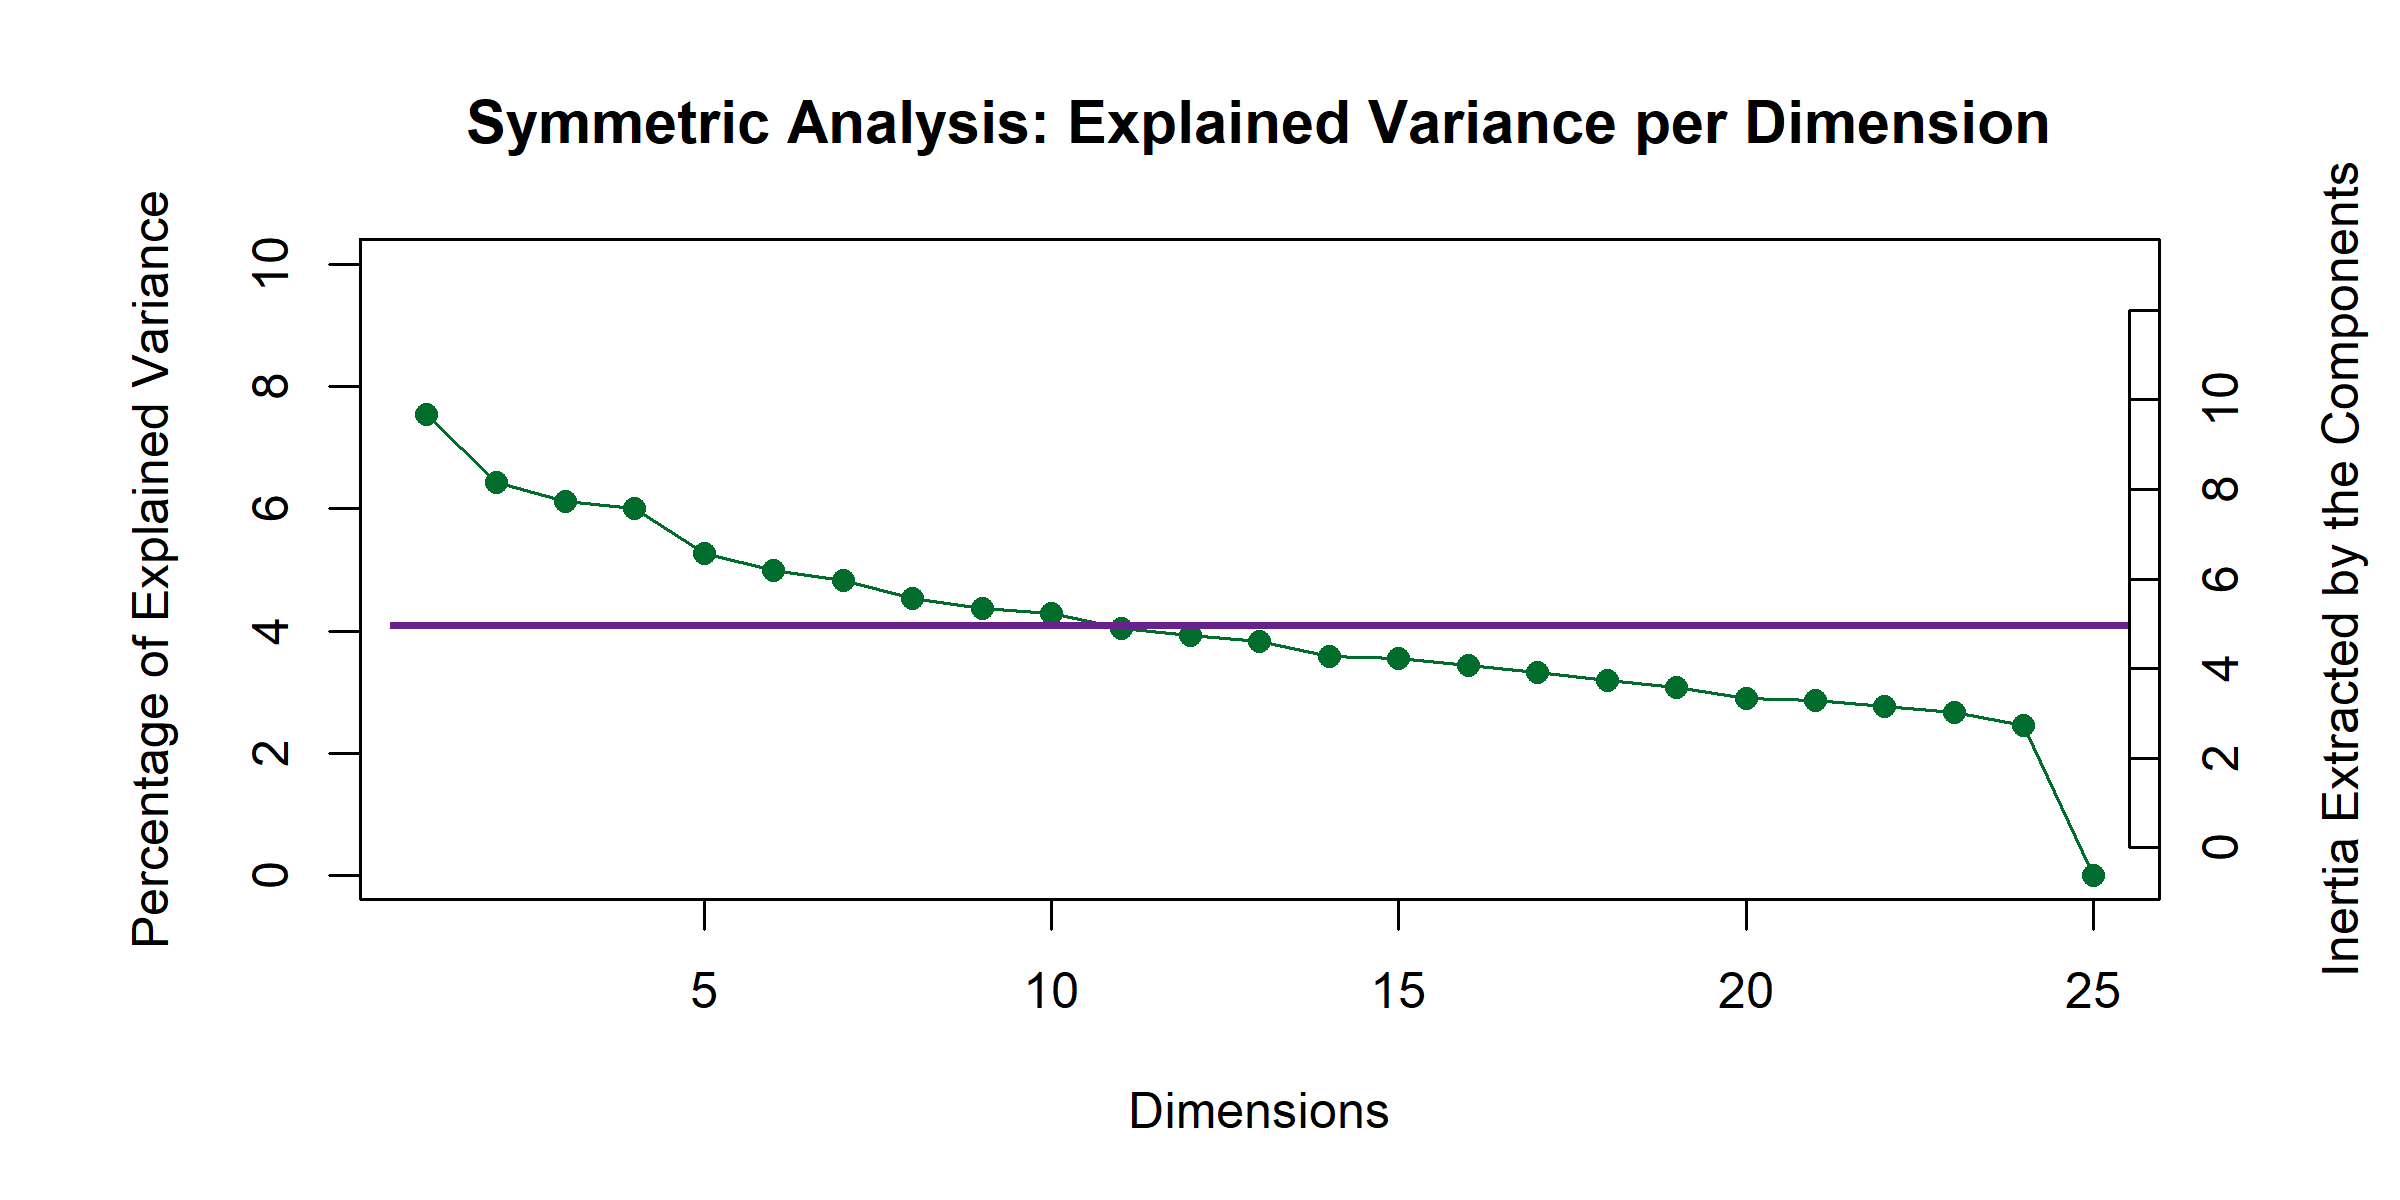
\includegraphics{./Music-Descriptor-Space_files/figure-latex/screeRV-1.png}
  \caption{ }\label{fig:screeRVQ}  
 \end{center}
\end{wrapfigure}

The scree plot in Figure \ref{fig:screeRVQ} shows the eigenvalues for the distance analysis between musical experts. For the purposes of this case study, we've opted to focus on the first two dimensions, which have \(\lambda\) = 9.06 and \(\lambda\) = 7.52, respectively. The fact that there are no dimensions that are exceptionally prominent suggests that each of the participants is contributing similarly to the dimensionality of this analysis, indeed, the first two dimensions only extract \textasciitilde13\% of the variance.\\
The MDS of the participants in this analysis revealed no significant differences between the experts based on any of the grouping variables used. The factor plots in Figure \ref{fig:judgesplotQ} show how the means of the factor scores, grouped by nationality and gender identity, respectively, are clustered on top of one another at the origin. The overlapping ellipses are the confidence intervals for the means. The individual data points are the same between the two plots, but the color of the dots, means and confidence intervals are different because they were calculated using different grouping variables.

\begin{figure}

{\centering 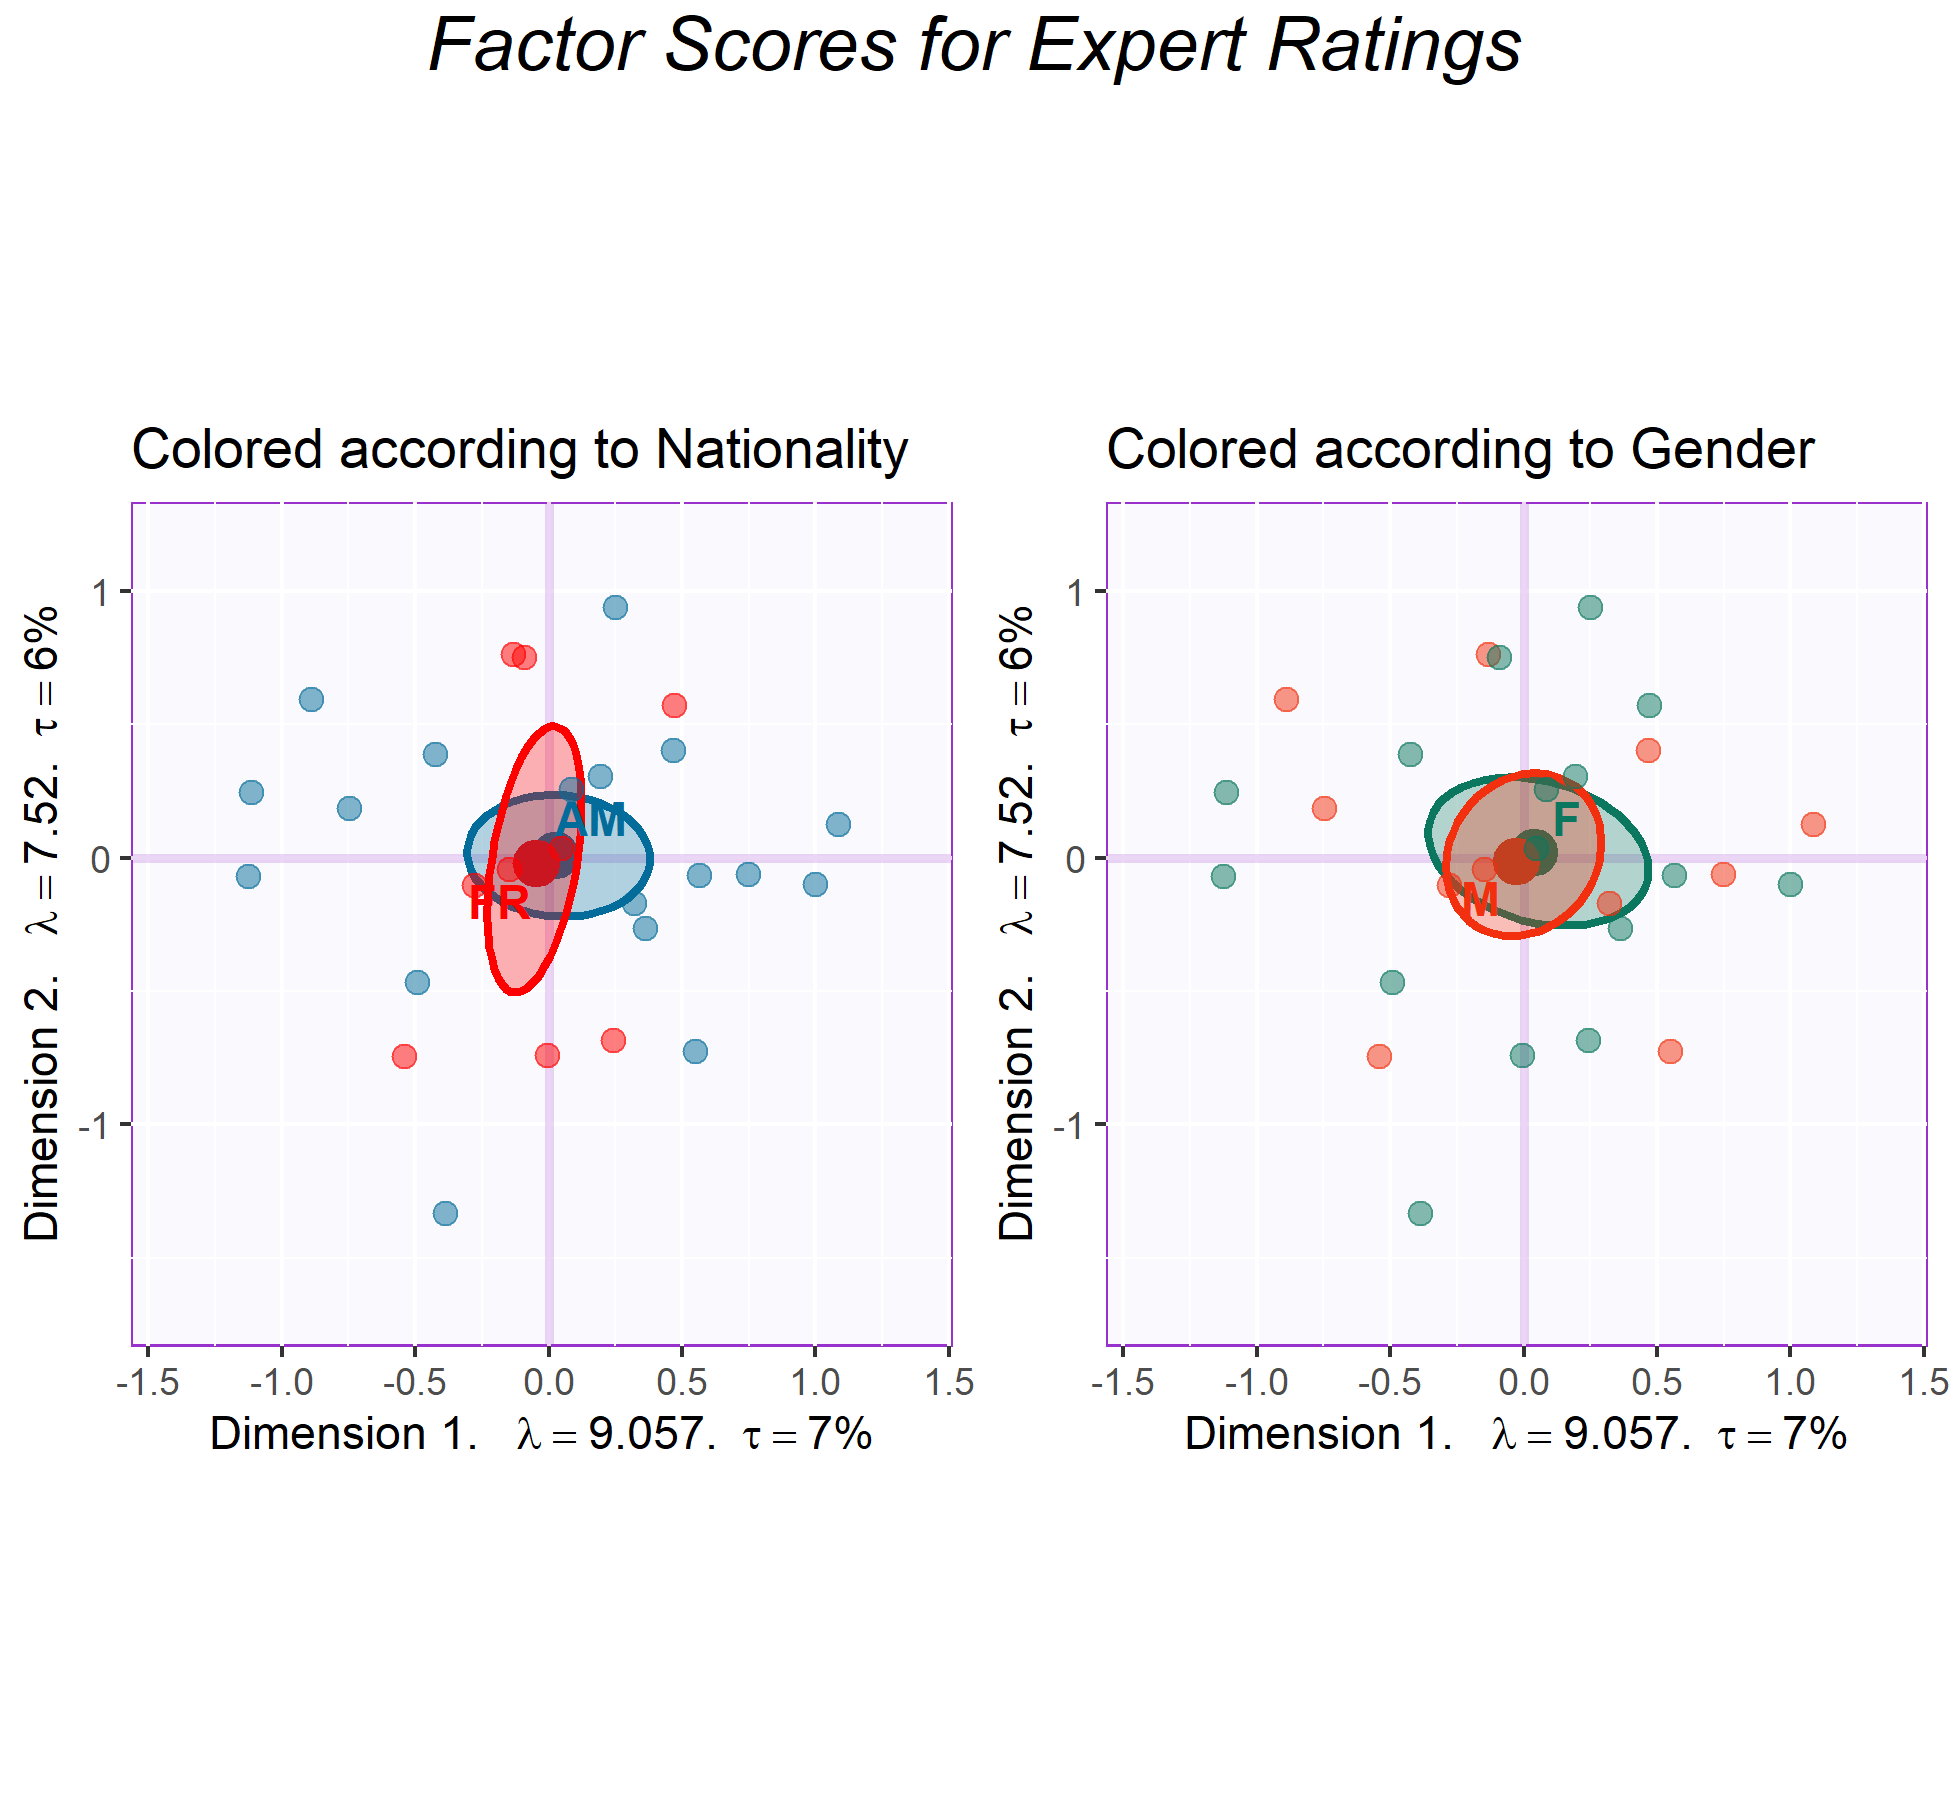
\includegraphics[width=0.75\linewidth]{Music-Descriptor-Space_files/figure-latex/judgesplotQ-1} 

}

\caption{ }\label{fig:judgesplotQ}
\end{figure}

\hypertarget{excerpts}{%
\subsubsection{Excerpts}\label{excerpts}}

\begin{wrapfigure}{h}{.5\textwidth}  
  \begin{center}
    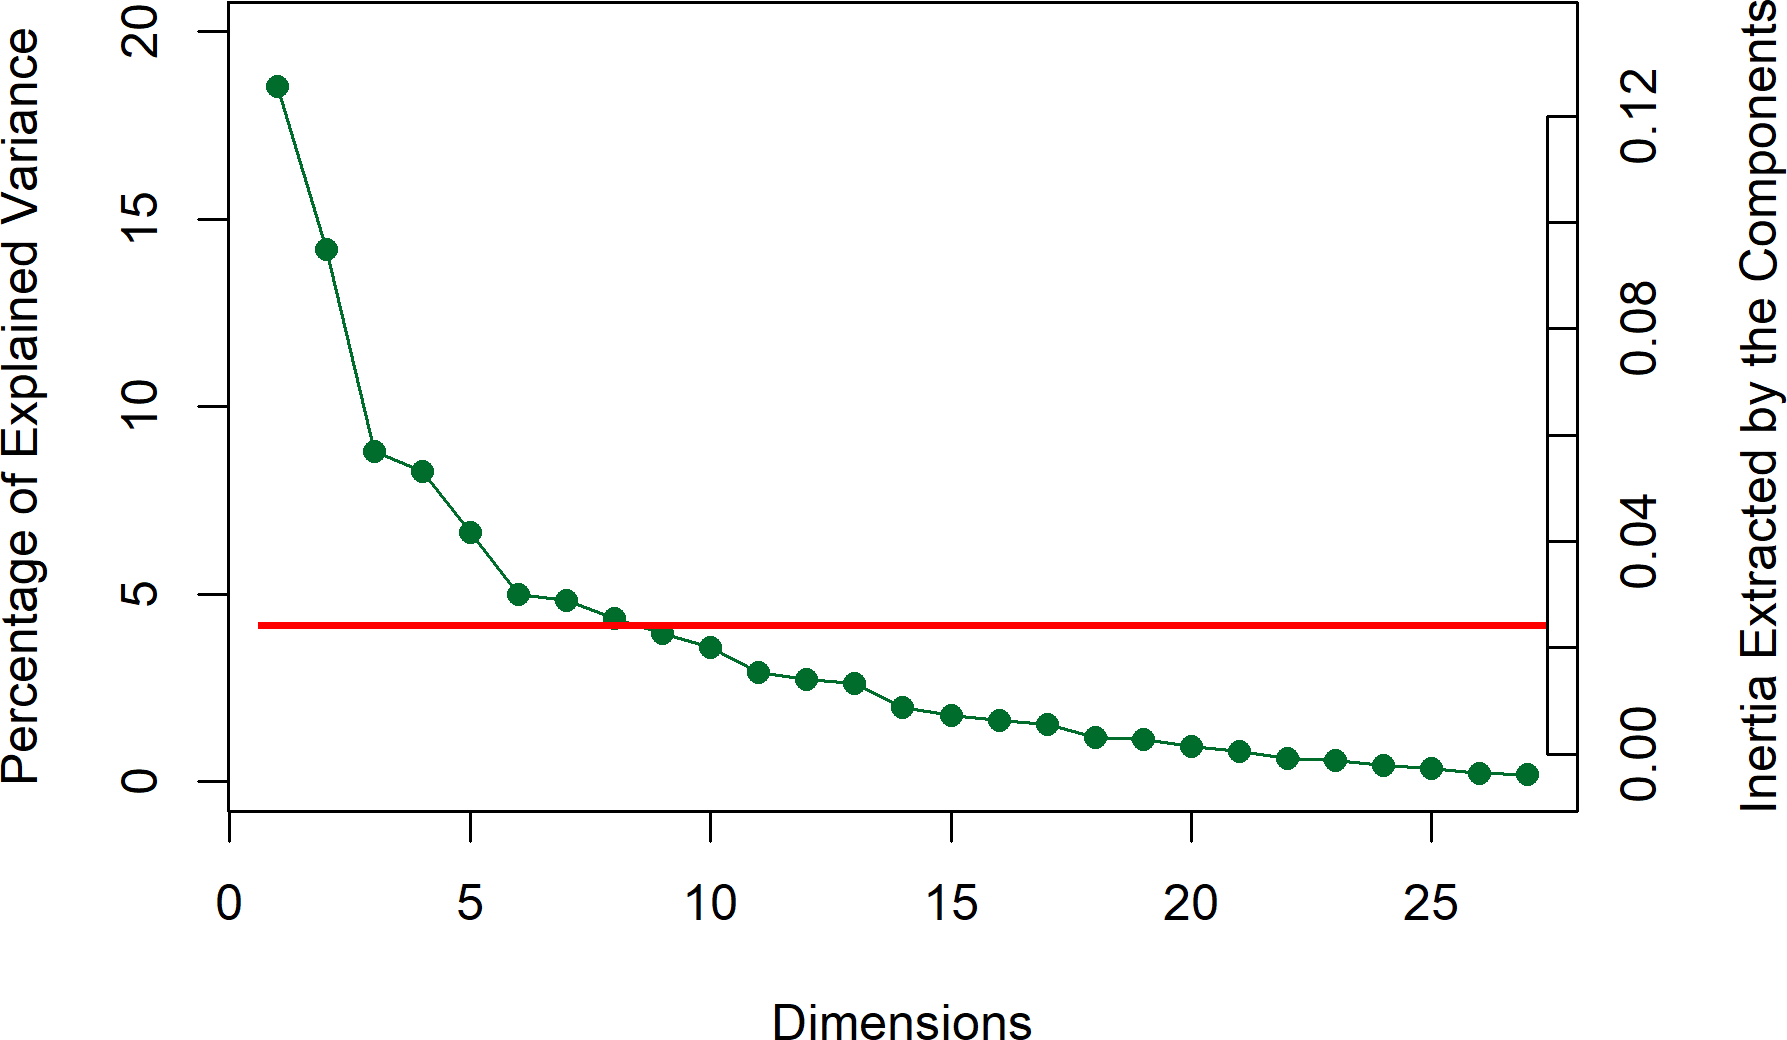
\includegraphics{./Music-Descriptor-Space_files/figure-latex/scree4excerptsq-1.png}
  \caption{ }\label{fig:scree4excerptsq}  
 \end{center}
\end{wrapfigure}

The scree plot for the analysis of the QS, Figure \ref{fig:scree4excerptsq}, shows the high dimensionality of this space, with the first four dimensions extracting a total of 49.63\% of the variance. Significant dimensions (i.e., dimensions that represent something other than noise) are indicated in purple. As stated above, for this case study, we focus on the first two dimensions.

Graphing the variable loadings (see Figure \ref{fig:contributionsQ}) of the musical qualities shows which qualities contribute the most to the first two dimensions (remember that the qualities are the variables in this analysis). Because of how CA is calculated, we know that the excerpts that load on the same dimension and direction as the musical qualities are the excerpts that are most associated with those qualities. The contributions shown here are only those that contribute significantly to the first two dimensions.
There are some obvious groups of variables, especially tempo and articulation in the first dimension, with fewer contributions from the dynamics group. The tempo variables load from high (tempo.F6 and tempo.F7) in the positive direction to low (tempo.F2 and tempo.F1) in the negative direction. Other contributions are one-off: major harmony, triple meter, classical genre, undulating contour, and disjunct motion. Because these one-offs don't show a clear pattern, it may be better to interpret these variables and their groups from the factor plots below. The excerpts are grouped according to the HCA performed on this data (see supplementary materials). Those that load positively, and are therefore associated with the qualities that load in the positive direction, are all from group 2: Excerpts 4, 13, 23, and 26. The ones that load in the negative direction are from mostly from group 4: Excerpts 7, 10, 24, and 27, with one from group 3, Excerpt 3.\\
The second dimension seems to dominated by a few groups: harmony, meter, genre, dynamics. The one-offs are slow tempo, ascending contour, and ``no melody.'' The excerpts that load significantly on this dimension are from all four groups. In the positive direction, we see Excerpts 7, 12, 15, and 27 from Group 4, and Excerpt 19 from Group 1. In the negative direction, Excerpts 2, 3, 11, and 17. All are from group 3 except for Excerpt 2, which is from Group 2. A full enumeration of contributions, loadings, and boostrap ratios is available from the author's github, for which the URL is in the author note.

\begin{figure}

{\centering 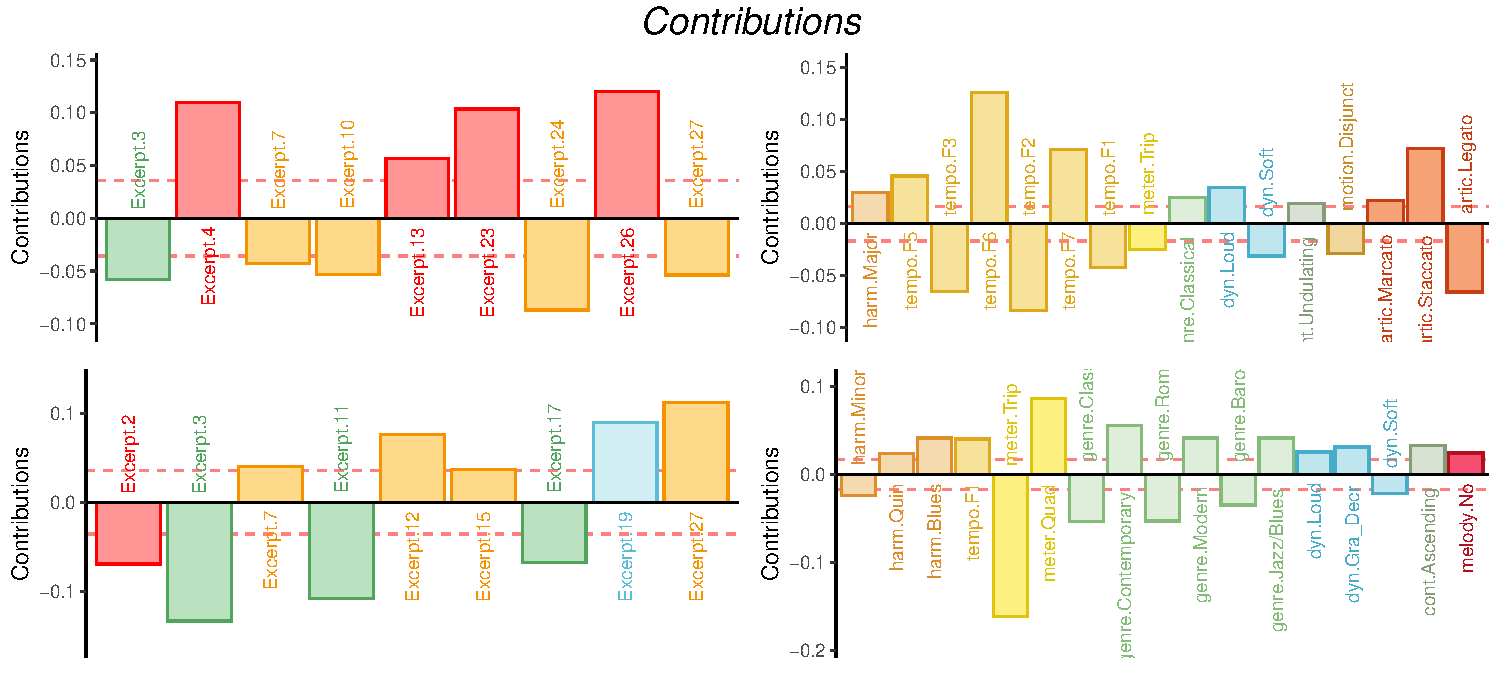
\includegraphics{Music-Descriptor-Space_files/figure-latex/contributionsQ-1} 

}

\caption{ }\label{fig:contributionsQ}
\end{figure}

\hypertarget{discussion}{%
\subsubsection{Discussion}\label{discussion}}

One assumption we make in an analysis like this is that the sample is random, which may not always be the case. The music itself is not random, as repetition is a common compositional tool, and was used in the composition of some of the excerpts. Perhaps more importantly, the excerpts were all composed by the same composer, which means that they are subject to the inherent biases of that composer, and some musical qualities are inextricably linked --- for example some harmonic elements with genre (Cohn et al., 2001). Additionally, although it is common practice to use pseudo-contingency tables in correspondence analyses, as we have done here, many of the values in this type of table are not random. Whereas, in a contingency table, there should be only a single one (1) per row, associating an observation with a single column or variable, a pseudo-contingency table like the one used here has more than one one (1) per row, meaning that those counts are linked and thus not random.

With regard to the scree plots in Figures \ref{fig:screeRVQ} and \ref{fig:scree4excerptsq}, there are a few guidelines on how many dimensions to interpret. One guideline, to analyze only dimensions with \(\lambda\) \textgreater{} 1, aren't helpful in either case, because all dimensions but one computed by the MDS have \(\lambda\) \textgreater{} 1 and all dimensions computed by the CA have \(\lambda\) \textless{} 1. Another is to apply the `elbow test,' to interpret the dimensions that fall above an inflection point in the scree plot. This option is not entirely conclusive in either case, either, for example in the CA, there are clear inflection points at dimensions three and six, and possible inflection points at eleven and sixteen. A third option is to analyze only dimensions that are greater than the average, indicated by the `Kaiser line,' in red, which would indicate that we should analyze as many as eleven dimensions for the MDS and eight dimensions for the CA. This is an excellent example of why permutation testing can help understand the dimensionality of a multivariate space. Even with permutation testing, however, we suggest as a guideline to analyze only the dimensions that are interpretable.

The graph depicted in Figure \ref{fig:factormapsQ} is a biplot depicting how excerpts and variables appear in the same mental space. This biplot is possible because of the nature of CA, but interpretation requires some discernment. The distance between the excerpts can be interpreted directly as similarity, and the distance between the musical qualities can be interpreted directly as similarity, but the distance between a quality and an excerpt cannot. Instead, the angle between an excerpt and a quality is indicative of their correlation. An angle of 0 indicates a correlation of 1, an angle of 90 indicates a correlation of 0, and an angle of 180 indicates a correlation of -1. See Abdi and Williams (2010a) for a more in-depth discussion of this.

Overall, this helps us to evaluate what qualities contribute to the excerpt groupings. These first two dimensions suggest that the hierarchical cluster analysis (see supplementary materials) revealed groupings roughly according to genre. However, there are two notable outliers. Preliminary versions of this analysis showed that Excerpts 6 and 14 dominated the 2nd and 3rd dimensions, respectively (see supplementary materials for visualizations). These two exerpts are unique in that they are each the only representative of their respective genres. Excerpt 6 is minimalist, à la Steve Reich, and Excerpt 14 is jazzy. In the plot below, they are included instead as supplementary projections, essentially `out of sample' elements.

Although they dominated the space when included in the sample, they are much closer to the barycenter of the plot when included as out of sample. Their placement indicates that the dimensionality of this space may in fact be related to musical genre or family. Were they to fall exactly on the origin, that would suggest that they shared no information whatsoever with the other excerpts included in the analysis. The disparity between their placement on the graph below and their placement on the graphs in which they are included in the main sample suggests that they share some information, but there is still a large amount of information that is not accounted for in the factor space depicted in Figure \ref{fig:factormapsQ}.

One perceptual element that is revealed here is that tempo and dynamics seem to contribute, intensity-wise, similarly to the first dimension. This points to two specific things. Firstly, it highlights possible bias in the compositional process. The excerpts were not intentionally composed with those characteristics being similar in mind, but it's entirely possible that the high or low arousal levels of the various excerpts that participants respond to also drove some of the compositional process, and that turned up in the results. Secondly, it's possible that the level of arousal was conflated between various musical qualities. For example, the intensity and therefore tempo of a stimulus may have been affected by the volume or dynamics (Kamenetsky et al., 1997). Perception of tempo is also affected by note rate or event density, which is also tied to arousal. In two pieces played at the same tempo, the one with more notes per unit time is more likely to be judged faster than one with fewer (Drake et al., 1999).

There are also a few musical elements revealed from the associations. The term staccato means short, or light and separated, and the term legato means smooth and connected. The participants in this experiment didn't have access to the notation, so they would be judging the excerpts aurally only. Between faster and slower excerpts, notes of the same rhythmic value take up less time in the faster excerpts, and may be more likely to be judged as light and separate, regardless of what the actual articulation was. Slow tempo and legato are associated differently. In terms of performance practice or pedagogy, slow notes are often intended to be connected as smoothly as possible, in order to create a sense of continuity. In terms of genre and harmony, many genres have harmonies associated with them (Kennedy et al., 2013), and the coordinate mapping of jazz/blues harmony and genre (on the third dimension) is the most extreme example of this. A glance back at the factor scores plot shows us more detail: the older styles, baroque, classical, and romantic, are negative on the 2nd dimension, as are the simpler harmonies of major and minor. Likewise the newer western styles, impressionist, modern, and contemporary, load positively on the 2nd dimension, along with the more complex harmonies of chromatic, whole tone, and ambiguous. A brief historical survey of the development of western harmony provides an interpretation for this. The classical genre has fairly structured rules for both harmony and voice leading, but the romantic era relaxed those rules and introduced more complex harmonies. The gradual devolution of those rules and the increase in complexity of harmony continued through the modern and contemporary styles (Kennedy et al., 2013). Historically speaking, the whole tone scale wasn't used commonly until the impressionist era (Cohn et al., 2001).

It is worth remembering, however, that because of the nature of this survey, these results tell us more about the perception of the excerpts themselves rather than the behavior of the participants. Because the excerpts were composed with the intent of varying across all of these musical dimensions, what we see is a sort of validation that there is, in fact, that variety among these excerpts, and that they are different enough to create a large and varied factor space.

\begin{figure}

{\centering 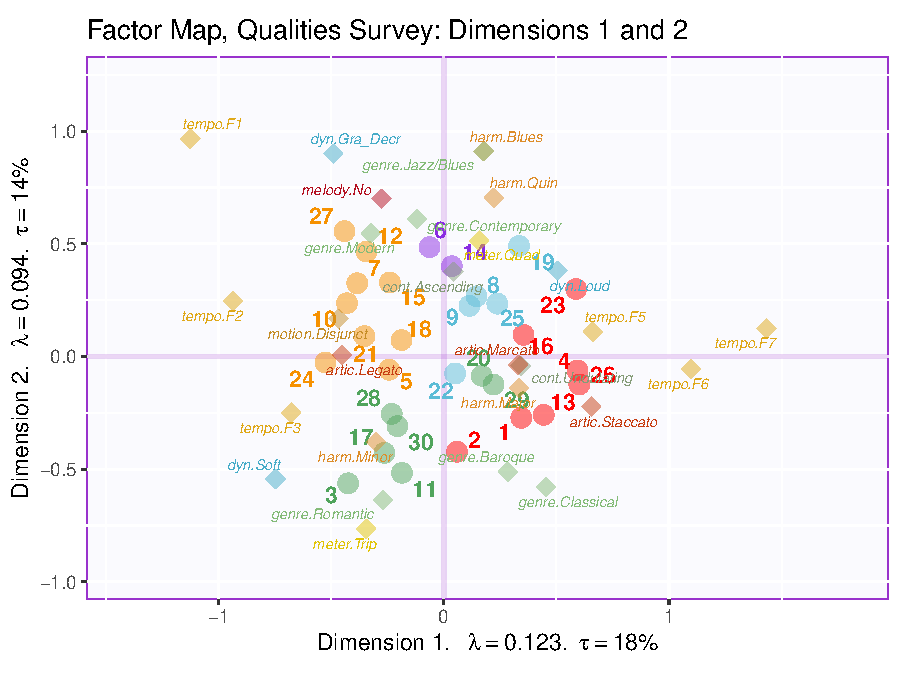
\includegraphics[width=0.75\linewidth]{Music-Descriptor-Space_files/figure-latex/factormapsQ-1} 

}

\caption{ }\label{fig:factormapsQ}
\end{figure}

\hypertarget{experiment-2-musical-adjectives-survey}{%
\section{Experiment 2: Musical Adjectives Survey}\label{experiment-2-musical-adjectives-survey}}

\hypertarget{methods-1}{%
\subsection{Methods}\label{methods-1}}

\hypertarget{participants-2}{%
\subsubsection{Participants}\label{participants-2}}

Participants with self-reported normal hearing were recruited for Experiment 2 without regard to level of music training. Participants in the United States were recruited through the UT Dallas Psych Research Sign-up System (SONA) and by word of mouth and social media. French participants were recruited by word of mouth, email, and social media. Only participants who signed up via the SONA portal were compensated with research participation credit, other participants were not compensated. Of a total of 520 survey responses, 160 were removed for not being incomplete, leaving a total of 360. Participants from the US who indicated a nationality other than American were excluded from analysis. ``Ghanian,'' for example, was not included, but responses such as ``Asian-American'' were. This left a total of 279 (\(\textit{N}_F\) = 108, \(\textit{N}_A\) = 171) survey responses for analysis. All recruitment measures were approved by the UT Dallas IRB.

\hypertarget{stimuli-1}{%
\subsubsection{Stimuli}\label{stimuli-1}}

The stimuli used for Experiment 2 are the same as those used for Experiment 1.

\hypertarget{surveys}{%
\subsubsection{Surveys}\label{surveys}}

Participants in Experiment 2 completed a survey (hereafter: Adjectives Survey/AS) via qualtrics in either English or French, depending on their location, that consisted of a CATA task in which participants evaluated the stimuli using adjectives. Thirty-three adjectives such as `dark,' `warm,' and `colorful' (French: `sombre,' `chaleureux,' and `colore'). The adjectives for the AS were selected using Wallmark (2019) as a guide and in consult with a French professional musician. Some adjectives were initially selected in French and some in English. In all cases, adjectives were selected for which there was a clear French (vis-à-vis English) translation. The adjectives are listed in English and in French in the supplementary materials. The survey also gathered demographic data, including age, gender identity, nationality, occupation, and musical experience.

\hypertarget{procedure-1}{%
\subsubsection{Procedure}\label{procedure-1}}

Participants were provided with a link to the survey and were instructed to listen to the excerpts presented in the survey either using headphones or in a quiet listening environment, but that was not controlled, nor was it assessed as part of the survey. After standard informed consent procedures, participants listened to 15 excerpts presented one at time in a random order, and answered a single CATA question per excerpt. All adjectives were presented, in a random order, for each excerpt. Demographic survey questions followed the experimental task.

\hypertarget{participants-3}{%
\subsubsection{Participants}\label{participants-3}}

\begin{wrapfigure}{h}{.5\textwidth}  
  \begin{center}
    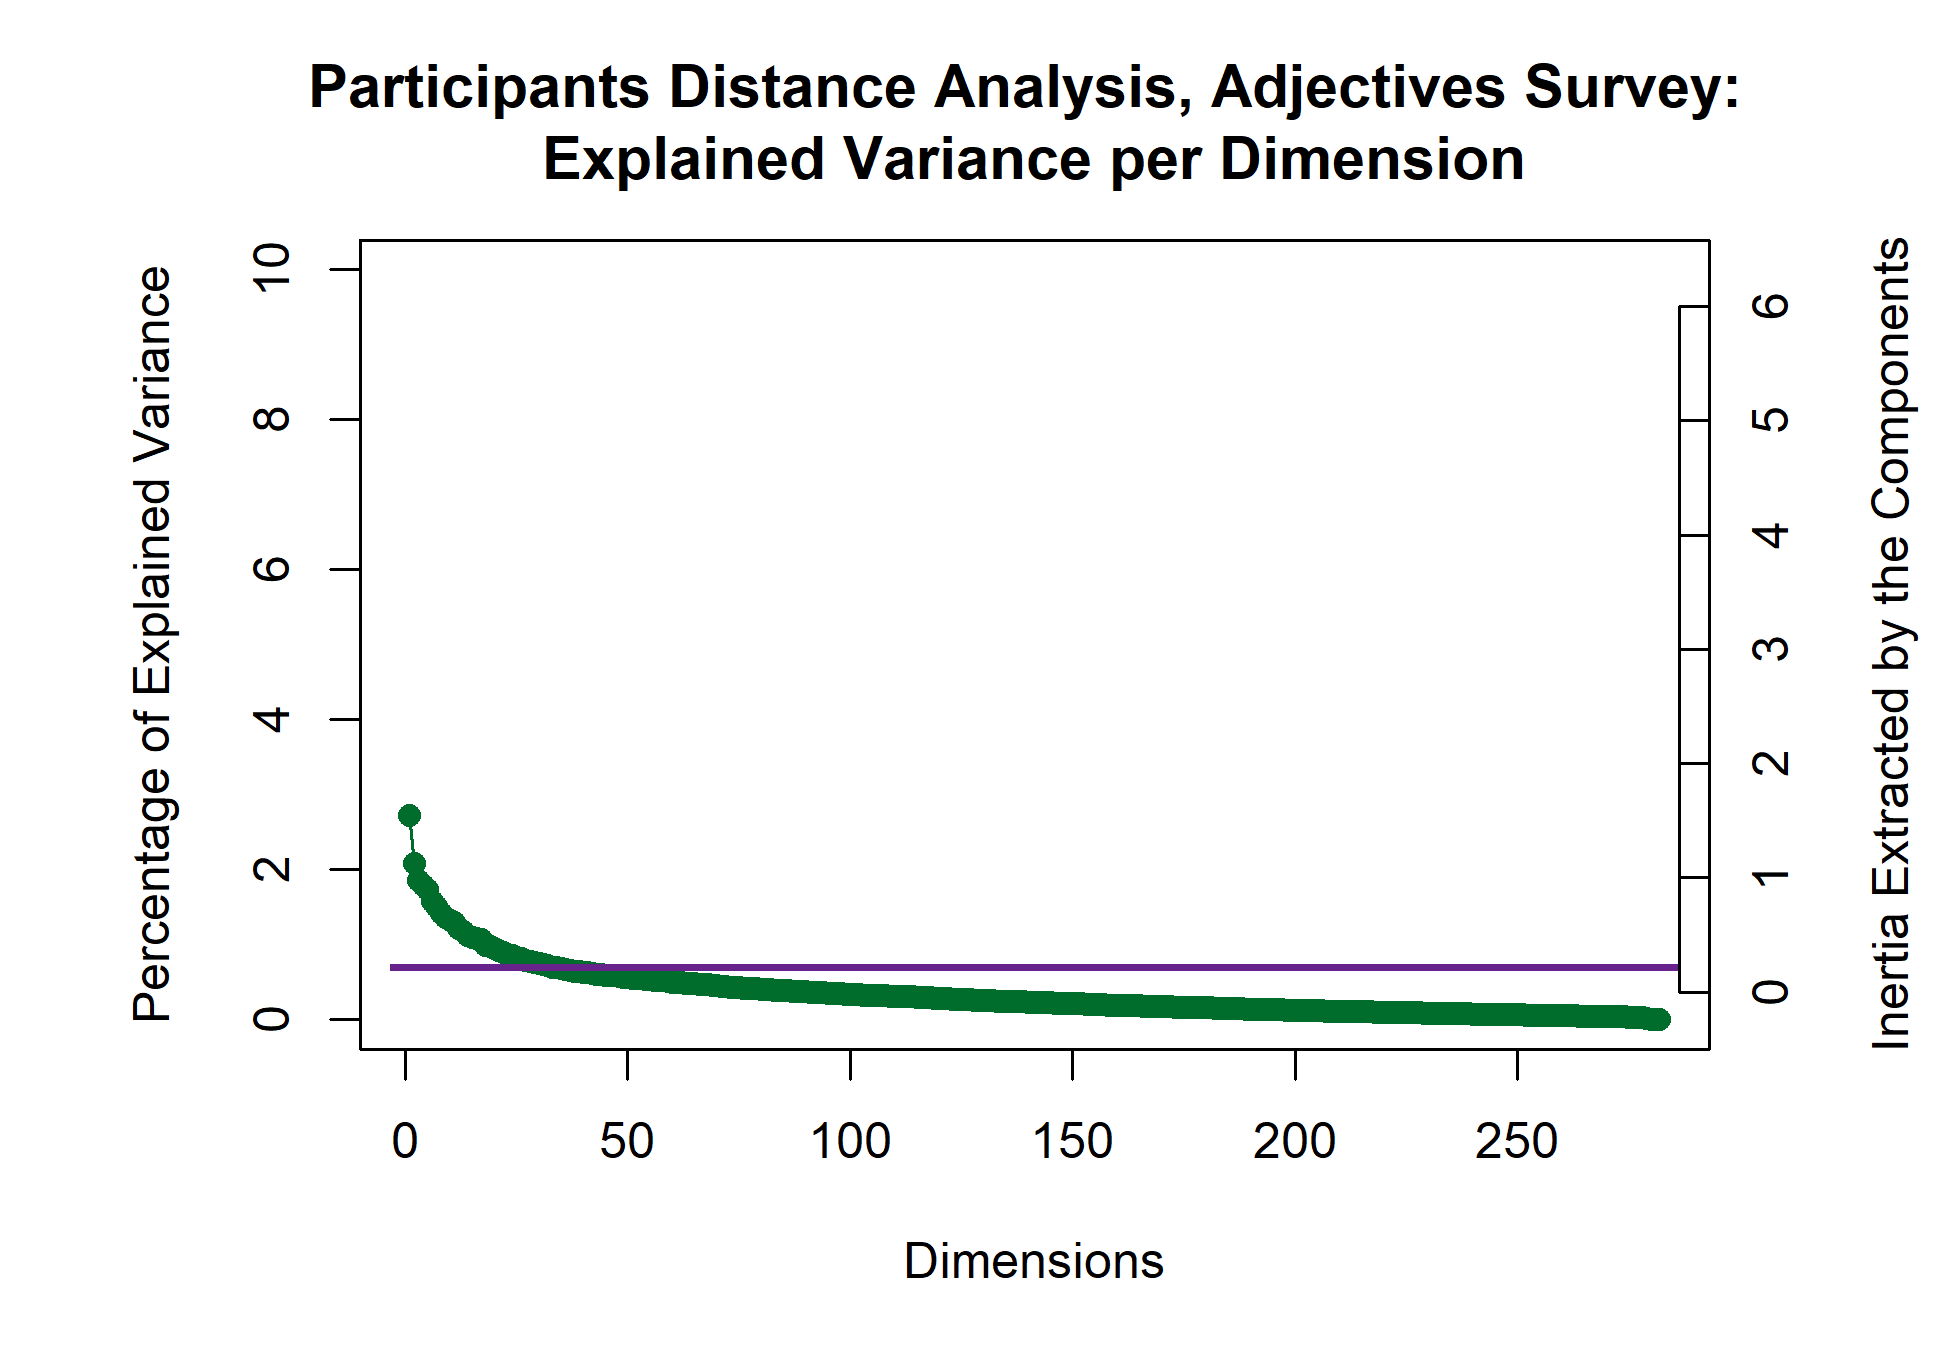
\includegraphics{./Music-Descriptor-Space_files/figure-latex/a.part.scree-1.png}
  \caption{ }\label{fig:apartscree}  
 \end{center}
\end{wrapfigure}

The scree plot depicted in Figure \ref{fig:apartscree} shows the explained variance per dimension for the distance analysis of participants in the adjectives survey. Again, having a high number of participants means that the dimensionality is high, and each dimension is only extracting a little variance. The first five dimensions all have \(\lambda\) \textgreater{} 1: 1.66, 1.27, 1.13, 1.09, and 1.06, respectively, but because of the high dimensionality here, the first dimension extracts only \textasciitilde3\% of the overall variance. Again, as above, for the purposes of this case study, we're focusing on the first two dimensions.\\
An MDS analysis of a distance matrix calculated from the pages of the brick revealed significant group differences in how French and American participants described the excerpts, \(\textit{p}\). \textless{} .01. The factor scores of the participants are plotted in Figure \ref{fig:map4RVA}, with with group means and bootstrapped confidence intervals shown for those means. The bootstrapping resampling was performed with 1000 iterations. We also analyzed the data using two other participant groupings as factors: gender identity, with three levels: Male, Female, or Non-Binary, and level of music training, with three levels: \textless{} 2 years, 2-5 years, and \textgreater5 years. Neither of these analyses revealed any significant differences between groups.

\begin{figure}   
  \centering  
  \caption{${R_V}$ Analysis of Participants in the Adjectives Survey}
    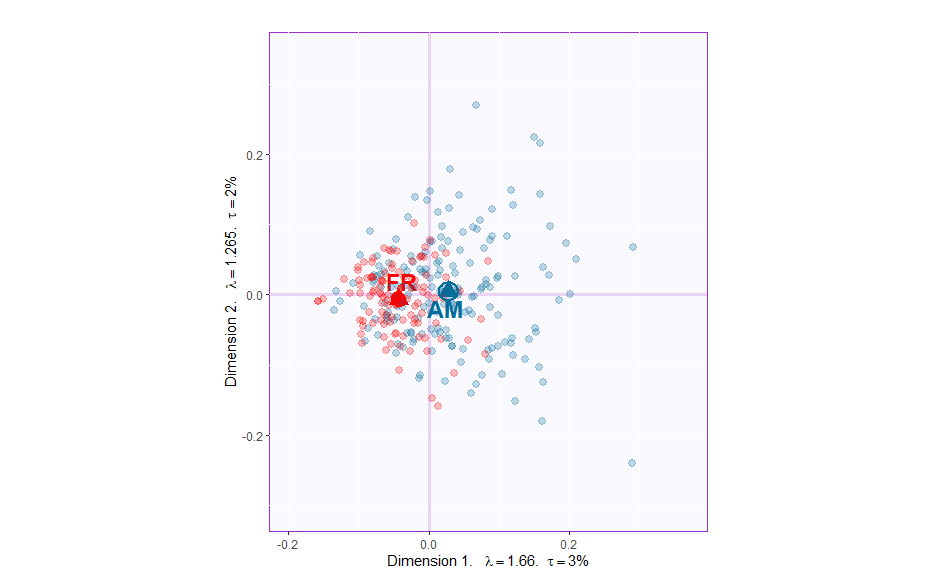
\includegraphics[width=0.7\columnwidth]{./Music-Descriptor-Space_files/figure-latex/apartrvmap.png}
  \label{fig:map4RVA}
  \caption*{\footnotesize \textit{Note.}  Group means are indicated with triangles and labled with AM and FR. The ellipse around the group mean indicates the confidence interval, after bootstrapping 1000 iterations. The fact that there is a clear separation between the group means and the confidence intervals suggests that there is a significant difference between the groups, \textit{p} > .001.}
\end{figure}

\hypertarget{excerpts-1}{%
\subsubsection{Excerpts}\label{excerpts-1}}

The plot in Figure \ref{fig:scree4descriptors} shows the explained variance per dimension in the analysis of the excerpts contingency table. Although there are no components with \(\lambda\) \textgreater{} 1, there are two strong dimensions that extract a majority of the variance. The first two dimensions extract 72.25\% of the variance, with the first dimension extracting a majority: 50.05\%, and the second dimension extracting almost a quarter of the overall variance: 50.05\%.

\begin{wrapfigure}{h}{.5\textwidth}  
  \begin{center}
    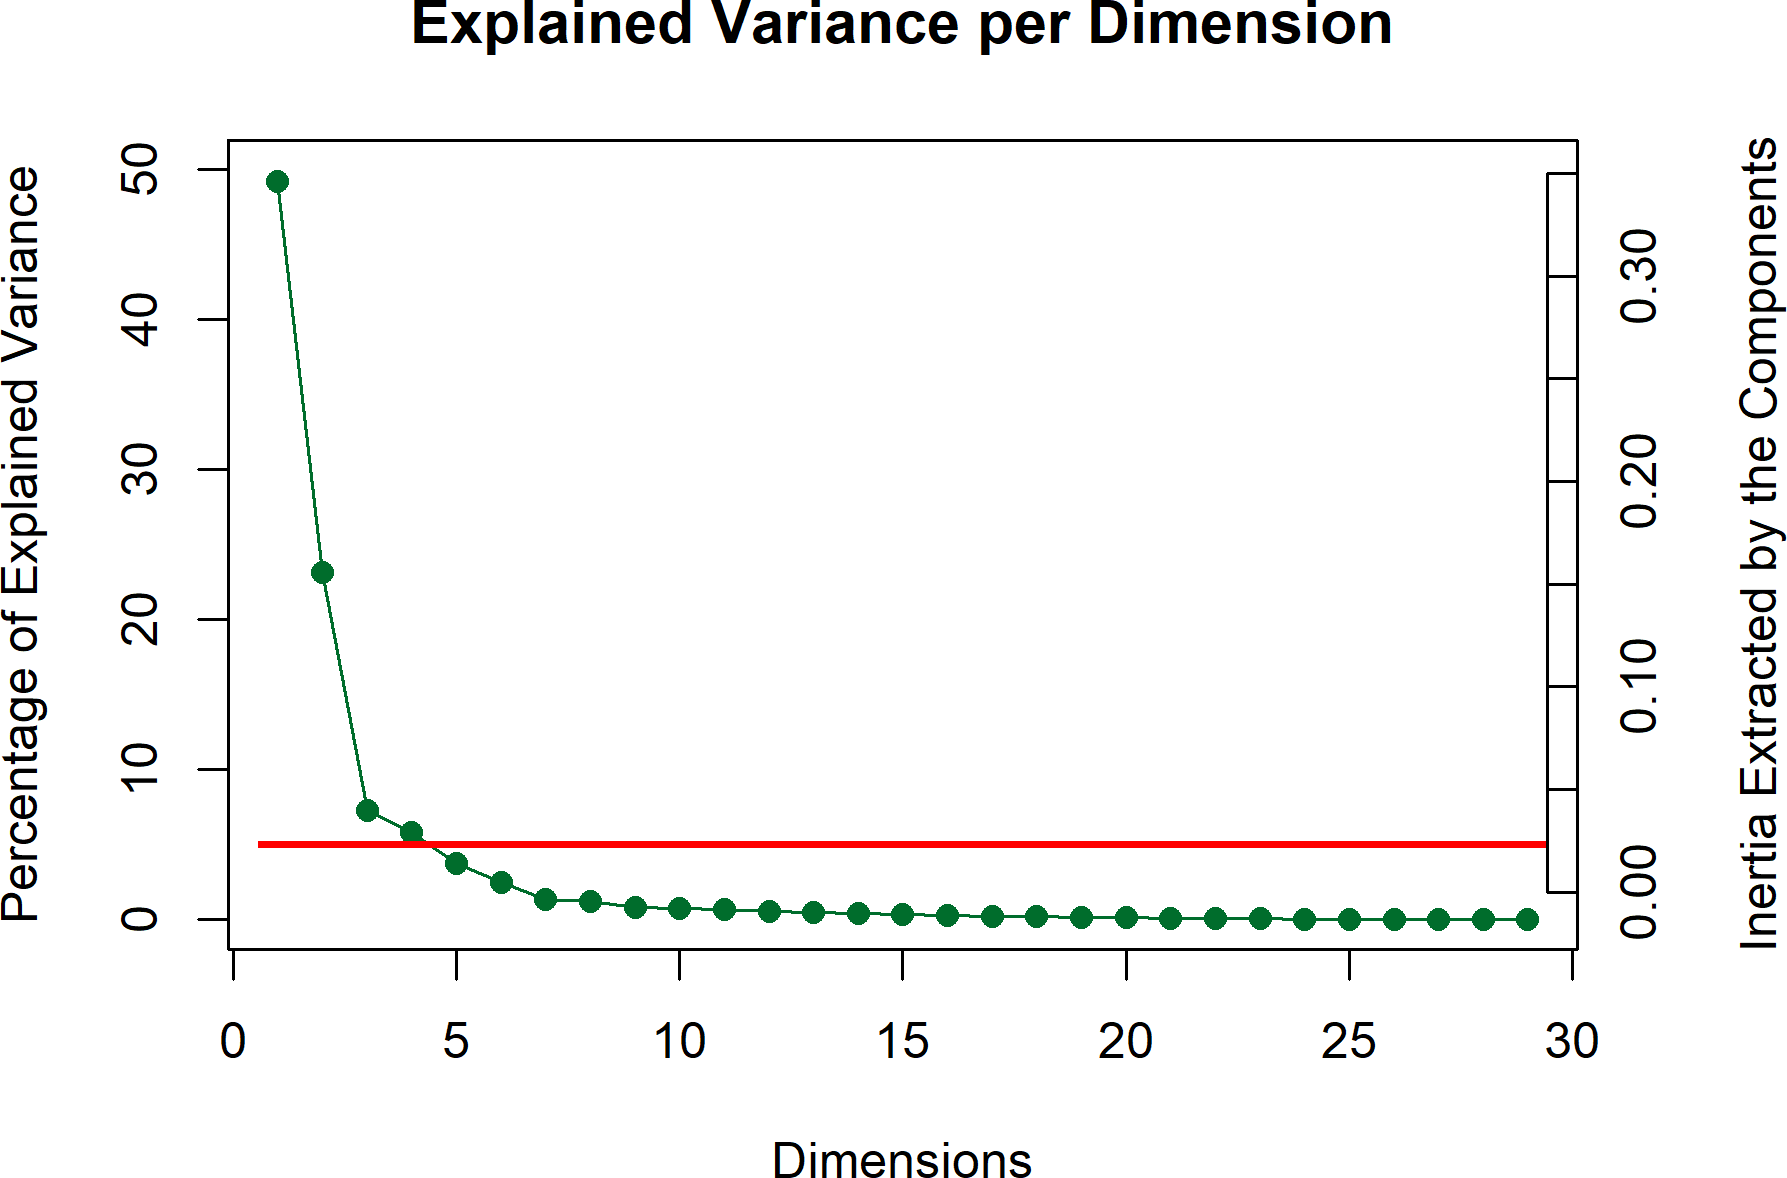
\includegraphics{./Music-Descriptor-Space_files/figure-latex/scree4descriptors-1.png}
  \caption{ }\label{fig:scree4descriptors}  
 \end{center}
\end{wrapfigure}

This plot also suggests that there are multiple `elbows,' at the 3rd, 5th, and 7th dimensions, respectively, with the third and fourth dimensions forming an `eigen-plane,' of two dimensions which extract similar amounts of variance and should be considered together. For this analysis, however, we're focused on the two first dimensions. Additionally, although excerpts 6 and 14 are outliers in the musical qualities survey, for reasons detailed above, they were not outliers in this analysis. We therefore included them in all of the analyses for Experiment 2.

The contributions to the first two dimensions are depicted in Figure \ref{fig:contributionsA}. Contributing significantly to the positive end of the first dimension are excerpts from group three (green) and to the negative end are excerpts from group one (yellow). Strong contributions on the positive end of the dimension from the adjectives ``Sad,'' ``Dark,'' ``Melancholy,'' ``Slow,'' ``Mysterious,'' ``Solemn,'' and ``Disturbing.'' The negative end of the first dimension is defined by the adjectives ``Fast,'' ``Happy,'' ``Dancing,'' ``Colorful,'' and ``Bright.''
The second dimension is dominated by excerpts from group 4 (red) in the positive direction and group 2 (blue) in the negative direction. Two excerpts from group 3 also contribute significantly, excerpts 7 in the positive direction and excerpt 10 in the negative direction. The columns contributing strongly in the positive direction are ``Aggressive,'' ``Fast,'' ``Disturbing,'' ``Mysterious,'' ``Surprising'' and ``Complex.'' The columns contributing in the negative direction are ``Warm,''Soft``,''Happy``,''Slow``,''Round``, and''Light".

\begin{figure}

{\centering 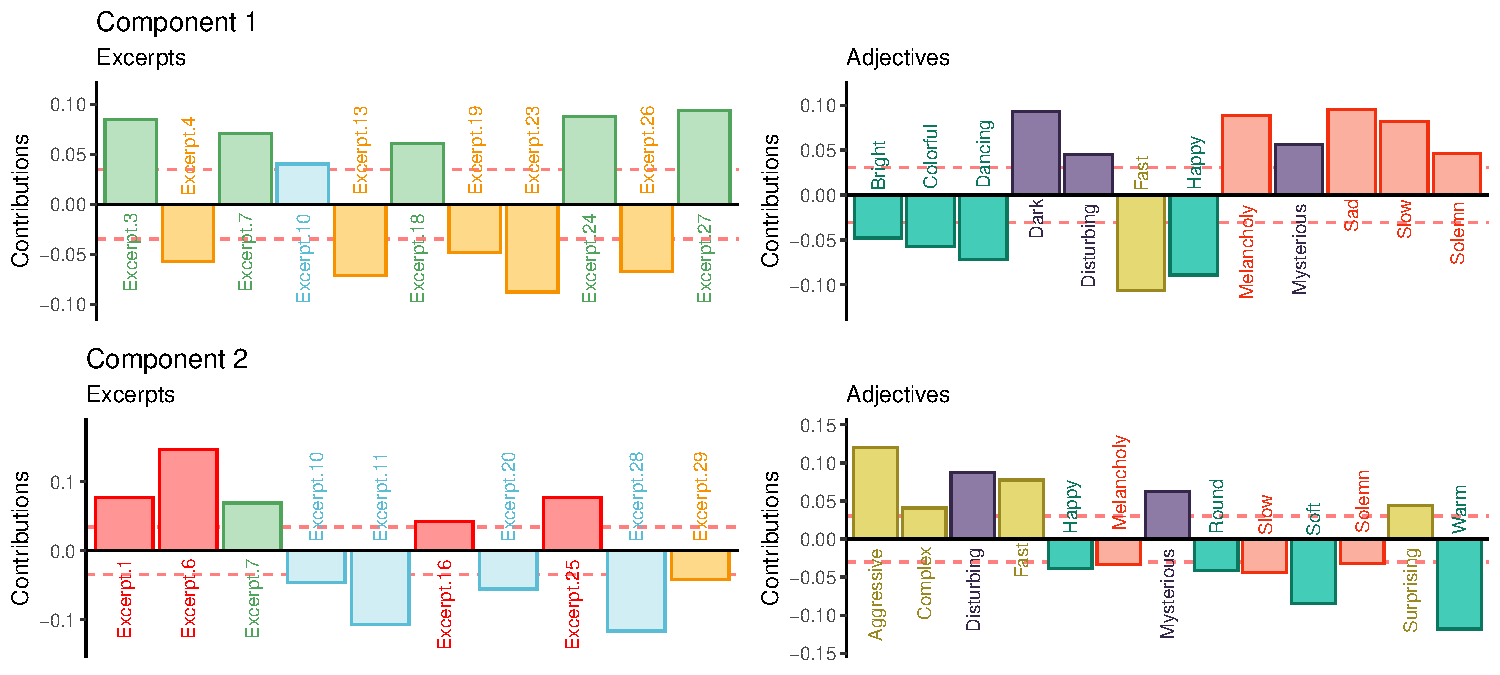
\includegraphics{Music-Descriptor-Space_files/figure-latex/contributionsA-1} 

}

\caption{ }\label{fig:contributionsA}
\end{figure}

The barplots in Figure \ref{fig:thebootsA} show the bootstrap ratios calculated for the rows and columns. Here we've included all of the rows and columns, because it's useful to see both which are significant and which are not. This is an inferential method that tells us is how consistently each of the observations and variables load on the first two dimensions. The threshold in this case is \emph{p} \textless{} .05. From this we get an idea of which of the rows and columns are stable, in other words, which ones tended to be rated in a certain way consistently across all participants, and also how likely these are to be observations reflective of the population as a whole. In this plot, the more extreme value of the bootstrap ratio, the more likely that it is a reflection of the `real' value. The values in the center of each plot that are grayed out identify the rows or columns that are not consistently loading on the dimensions. With the observations and variables ordered like this, it makes it easy to see how the consistently the clusters are distributed in the space. This plot was not included for Experiment 1 because it would be less informative given what the survey in Experiment 1 was assessing. Experiment 1 doesn't evaluate the behavior of participants, but the nature of the excerpts.
Note that there are far more significant bootstrap ratios than there are significant contributions. That just means that while not everything is contributing, overall the model seems to be stable. Fewer significant bootstrap ratios would suggest that there was a greater amount of variance in the observations and variables than were accounted for, at least in the first two dimensions. Looking at the nonsignificant values for the adjectives may inform our understanding of the participants' use of the adjectives. `Incisive,' `transparent,' `poweful,' `dense,' `round,' and `sparse,' are all nonsignificant on the first dimension, and `weak,' `dull,' `sparse,' `valiant,' and `short' are all nonsignificant on the second dimension. All but `sparse' are significant on one dimension or the other. Looking at the column sum for `sparse' tells us that it was used, so this isn't an effect of participants not using this word. It's more likely that `sparse' doesn't really fit into the Valence-arousal plane. It's a neutrally valenced word that could describe excerpts that fall anywhere within that plane. `Weak' and `transparent' give us another important perspective. These were the two least commonly used adjectives, but the fact that they are consistently loading on one dimension or the other suggests that when they were used, they were used in the same way.

\begin{figure}

{\centering 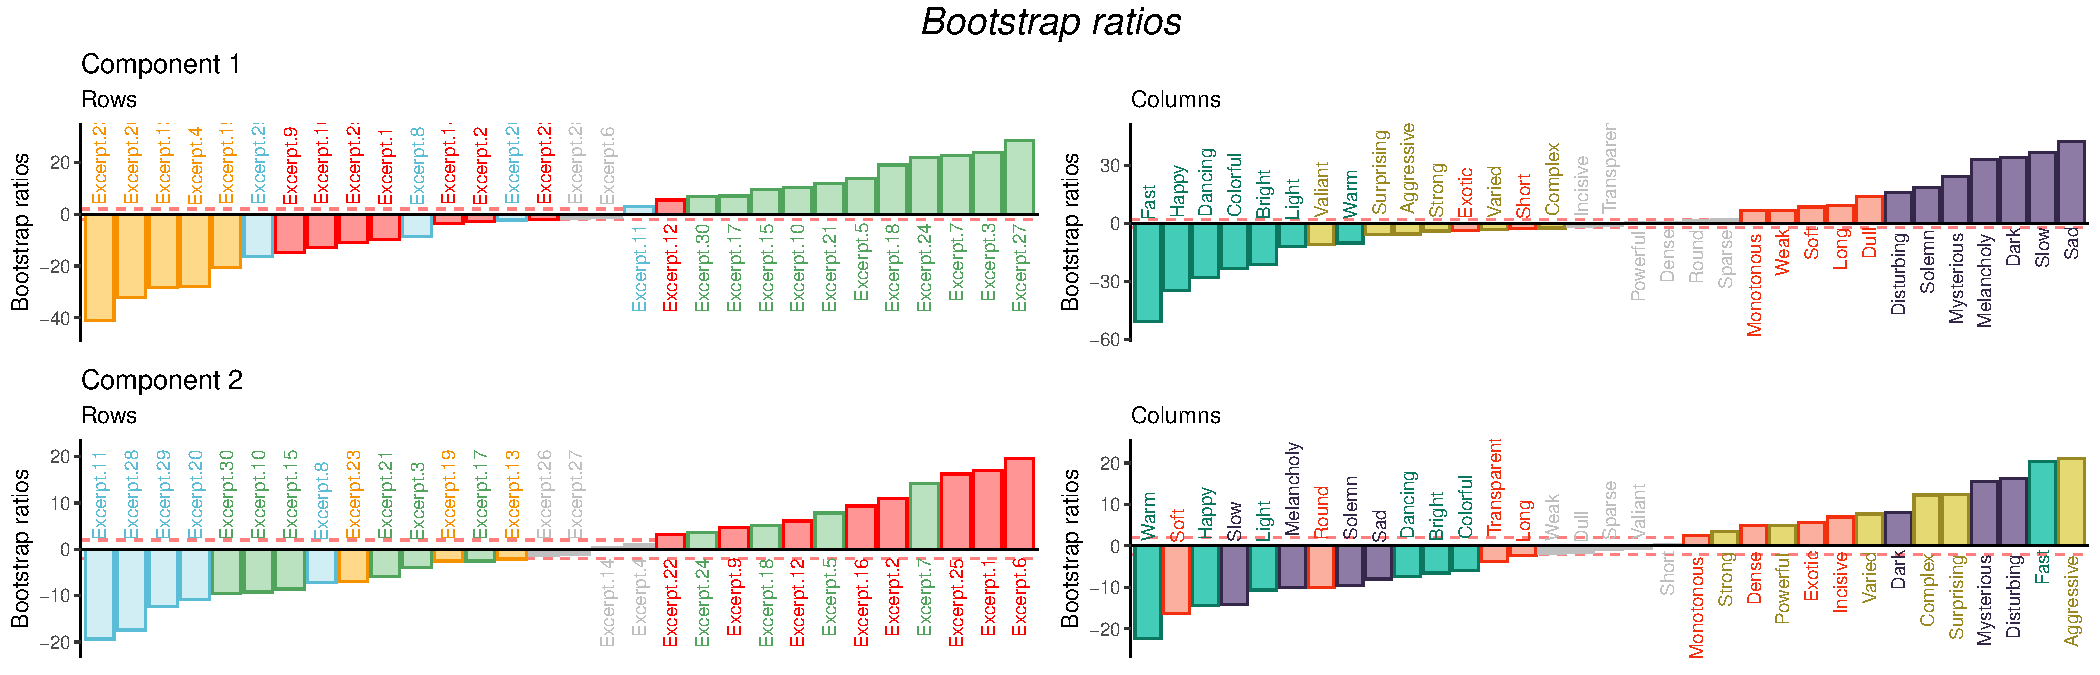
\includegraphics{Music-Descriptor-Space_files/figure-latex/thebootsA-1} 

}

\caption{ }\label{fig:thebootsA}
\end{figure}

\hypertarget{discussion-1}{%
\subsubsection{Discussion}\label{discussion-1}}

The factor maps below show the row and column factor scores for the American and French participants. These are once again symmetric plots, interpretation is the same as the factor plot for the musical qualities. There's a clear valence-arousal plane apparent for both, and in both cases valence seems to define the first dimension and arousal defines the second dimension. However, the difference in the amount of variance extracted by the first two dimensions between the French and American participants is notable. The French data show a weaker first dimension but a stronger second dimension relative to the Americans, both in terms of variance extracted (tau), effect size (lambda). This tells us that French participants were less affected by the excerpts than the American participants, but they responded more to the arousal of the excerpts.
There are also differences in how the adjectives and the excerpts are distributed in the space. One clear example is that Excerpt 6 is in quadrant two in the American plot, but quadrant one in the French. This is a small change, but it suggests that the French participants were more likely to assign negative valence to this excerpt, and American Participants were more likely to assign positive valence. For the adjectives, `bright' and `dancing' are directly on top of one another in the American plot, but there is some space between the two in the French plot. It's possible that this reflects the idea that although the meaning is shared between languages, there are semantic or associational differences between the words.

\begin{figure}   
  \centering  
  \caption{Symmetric Plots for Rows and Columns of the Adjectives Surveys, by Participant Nationality}
    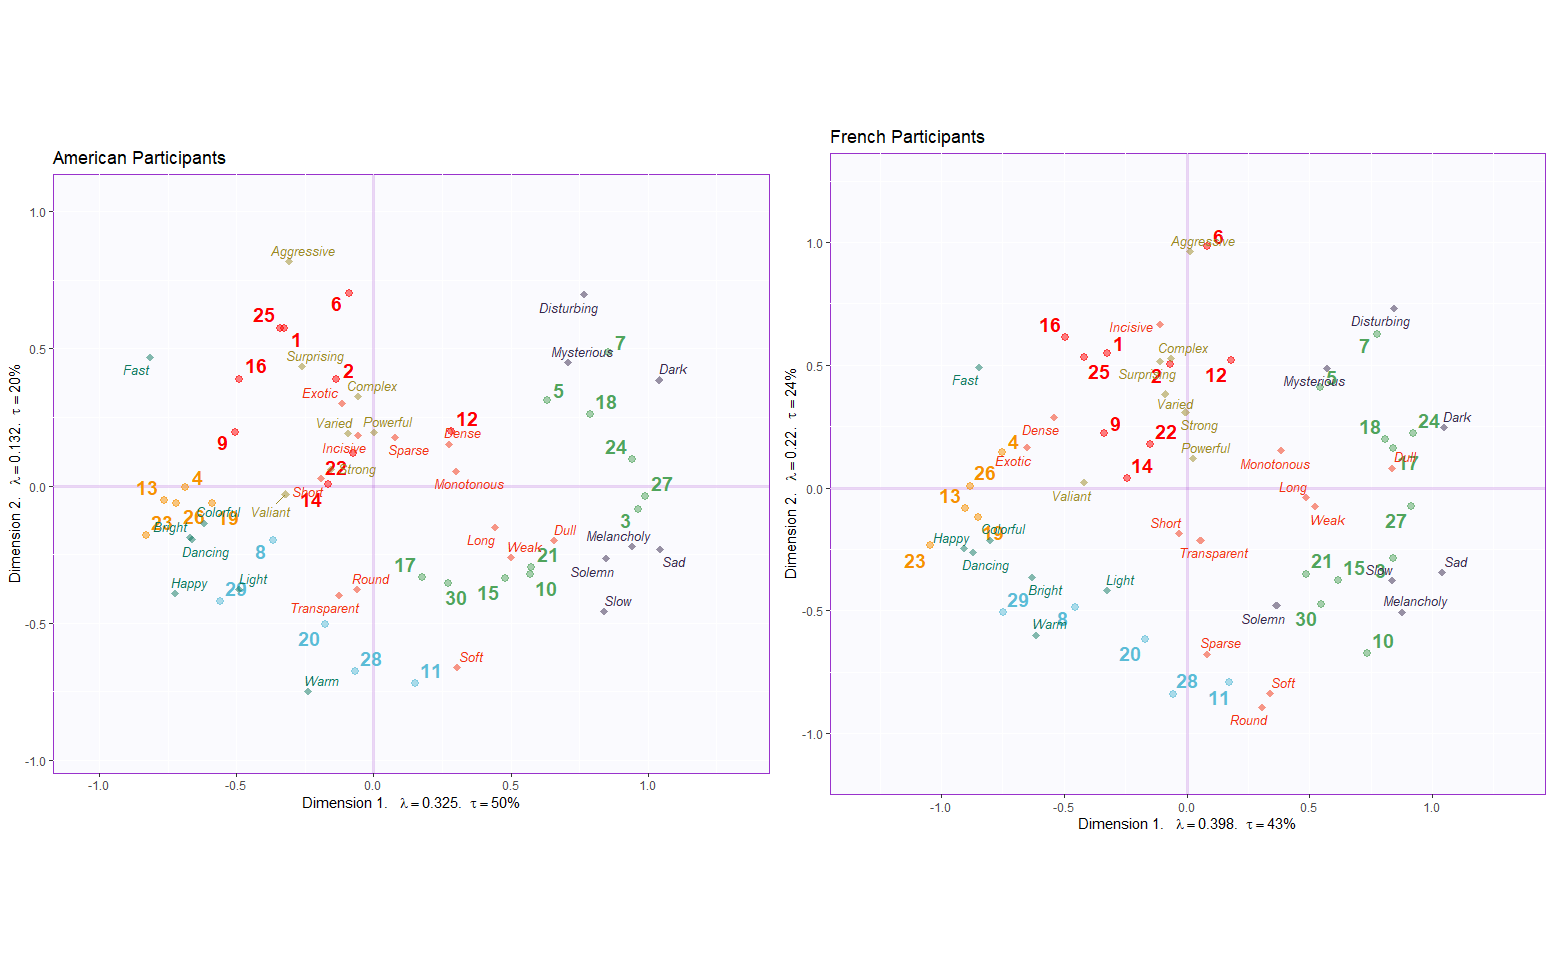
\includegraphics{./Music-Descriptor-Space_files/figure-latex/factormapsA.png}
  \label{fig:factormapsA}
  \caption*{\footnotesize \textit{Note.}  For these plots, the survey responses were split by nationality and analyzed separately. Note the differences in variance extracted by each of the first two dimensions.}
\end{figure}

Another way to visualize the relative contributions of the groups to the factor space is to use an MFA, the results of which are displayed in Figure \ref{fig:mfasbs}. In these plots, we can see the differences in behavior between the groups more clearly. A few examples of excerpts that were rated differently are Excerpts 6, 8, 12, and 17. Words that were used differently include ``Disturbing,'' ``Round,'' ``Solemn,'' and ``Bright.'' It appears that the valence-arousal plane uncovered in the CA is also present here, and this provides a framework for interpreting the differences in behavior between the groups. Excerpt 17 is perhaps the most extreme example. American participants rated this excerpt with much lower arousal and slightly less negative valence than the French participants, so much so that for the American participants, the excerpt landed in the ``low arousal/negative valence'' quadrant, and for the French participants it landed in the ``high arousal/negative valence'' quadrant. Another interesting case is for Excerpt 8, which lands in the same quadrant for both groups, but much further from the origin for the French participants than the Americans. The way in which the two groups used the words is also curious. For example, Disturbing seems to be more extreme for the French participants than the Americans. On the other hand, ``Solemn'' seems to be more a function of arousal in French and valence in English. ``Bright'' is another example of a word that seems to have the same intent but different extremity between cultures. For American participants, ``Bright'' seems to carry much more positive valence than for French participants.

\begin{figure}
     \centering
     \caption{Partial Factor Scores Plots from the MFA}
     \begin{subfigure}[b]{0.49\textwidth}
         \centering
         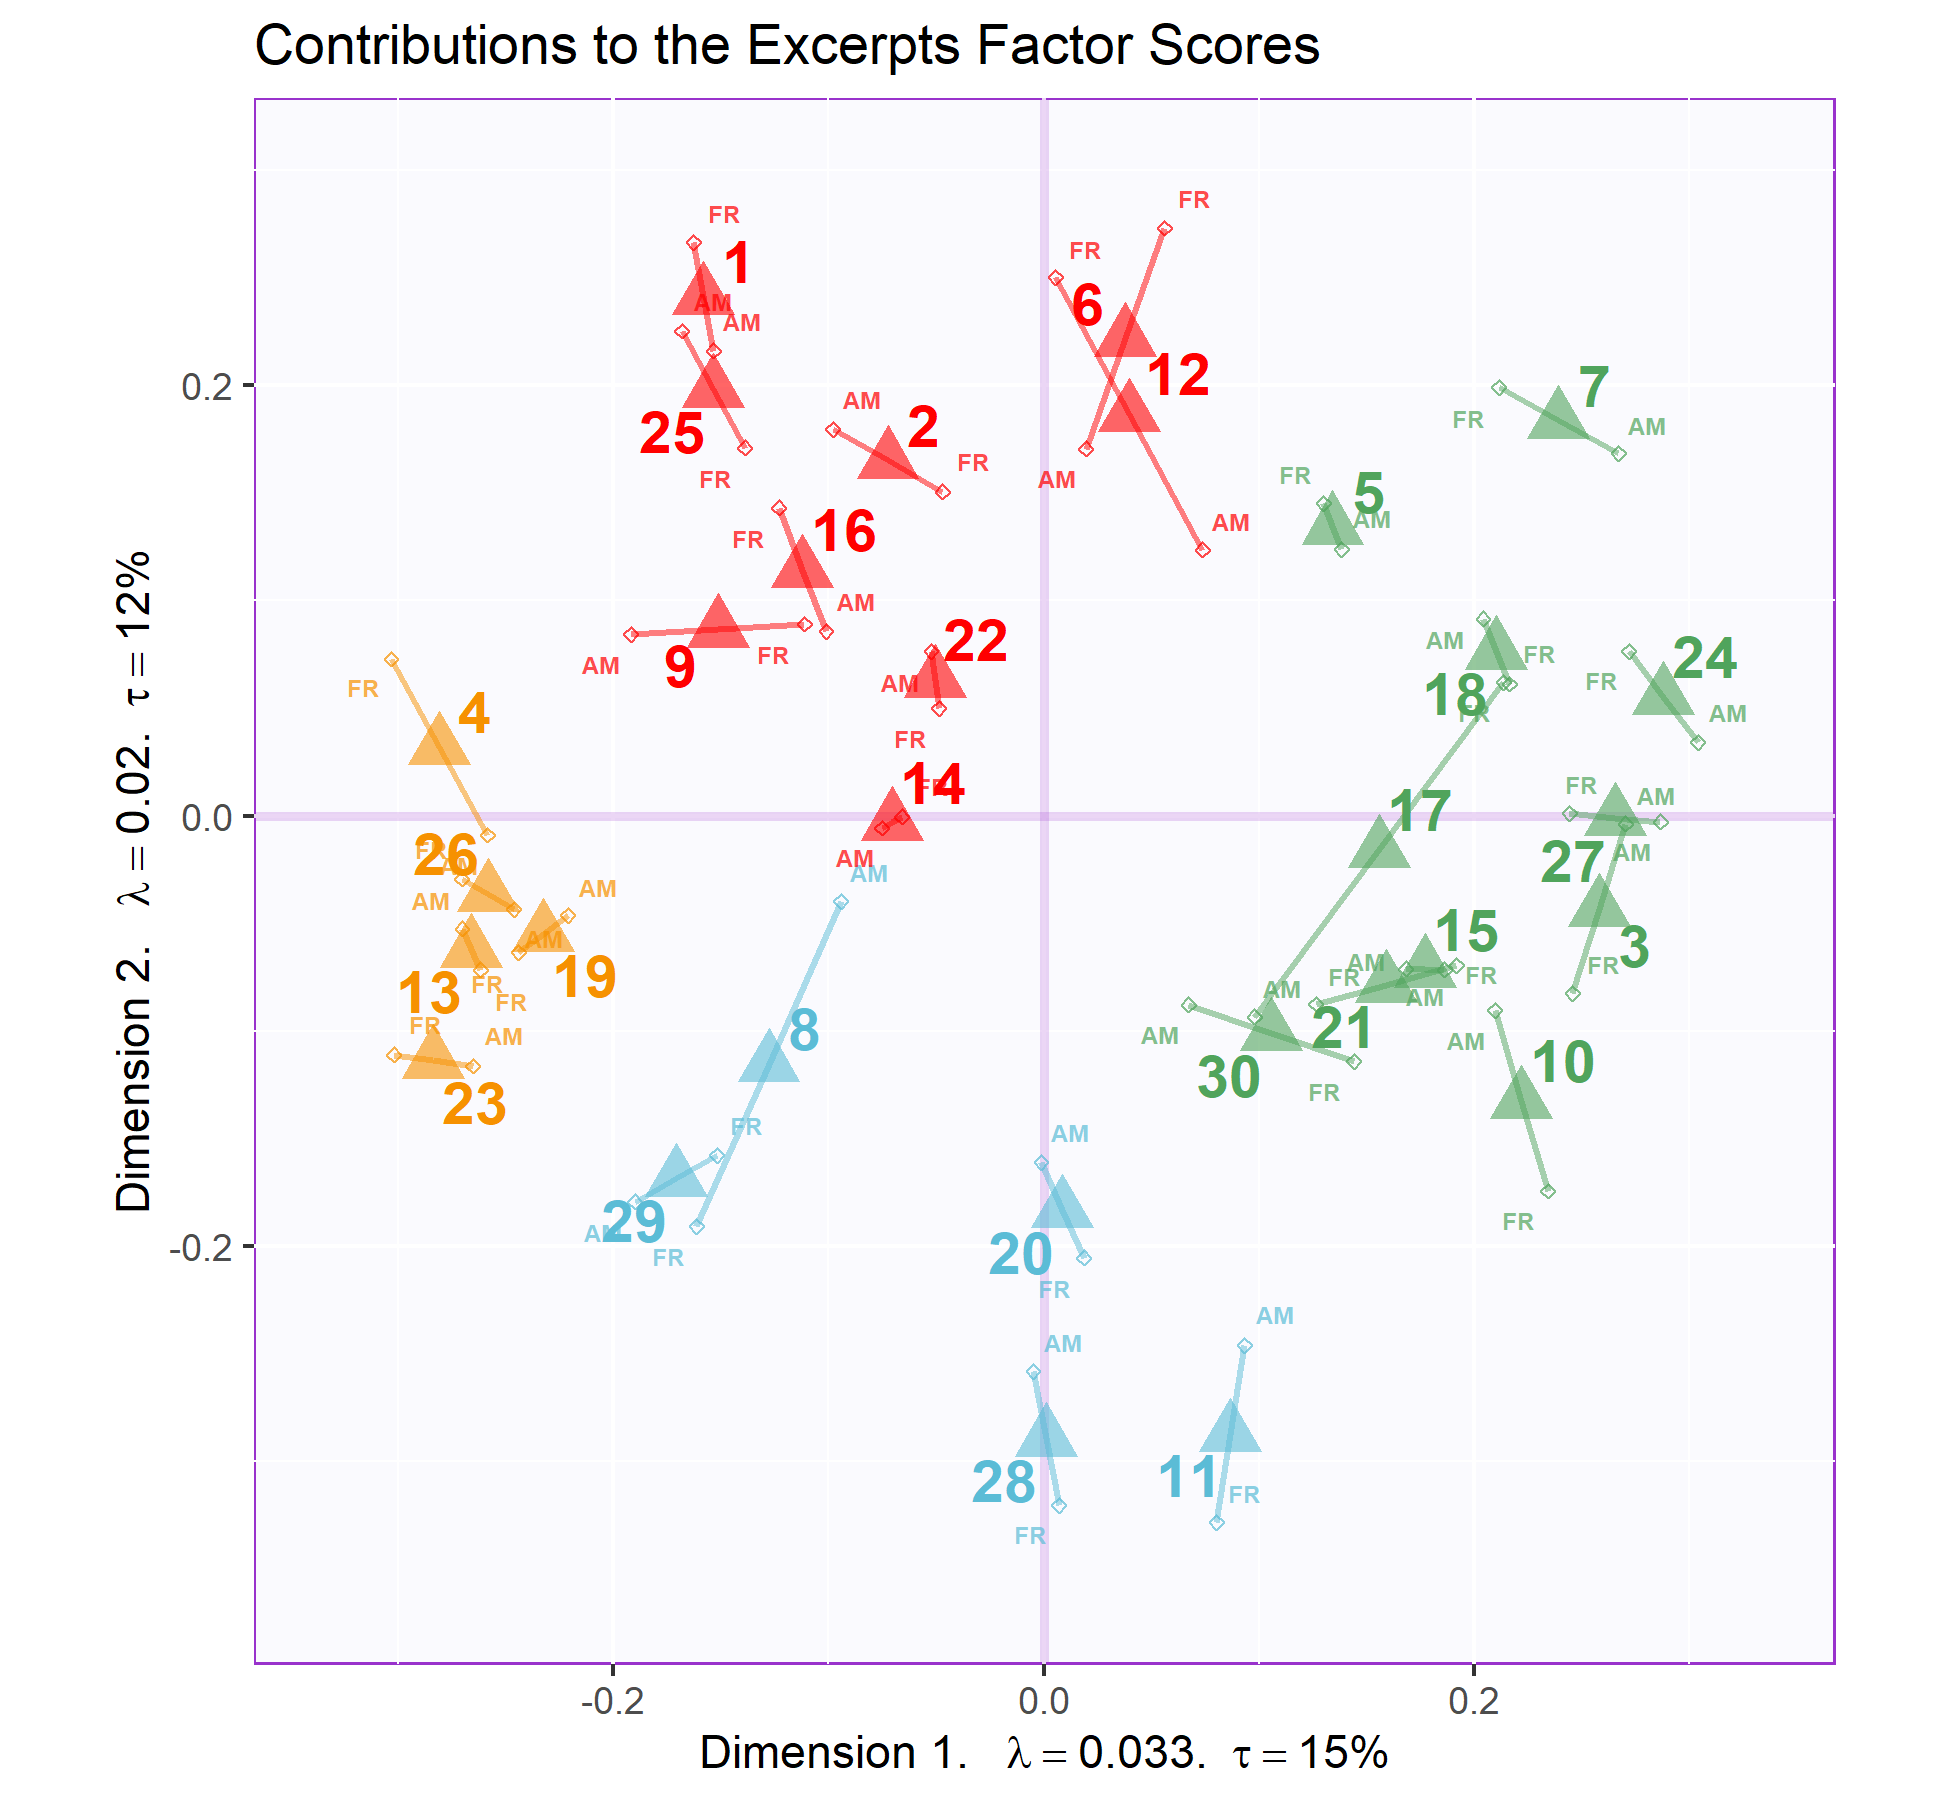
\includegraphics[width=\textwidth]{./Music-Descriptor-Space_files/figure-latex/mfasbs-1}
         %\caption{$y=x$}
         \label{fig:excerptspfs}
     \end{subfigure}
     \hfill
     \begin{subfigure}[b]{0.49\textwidth}
         \centering
         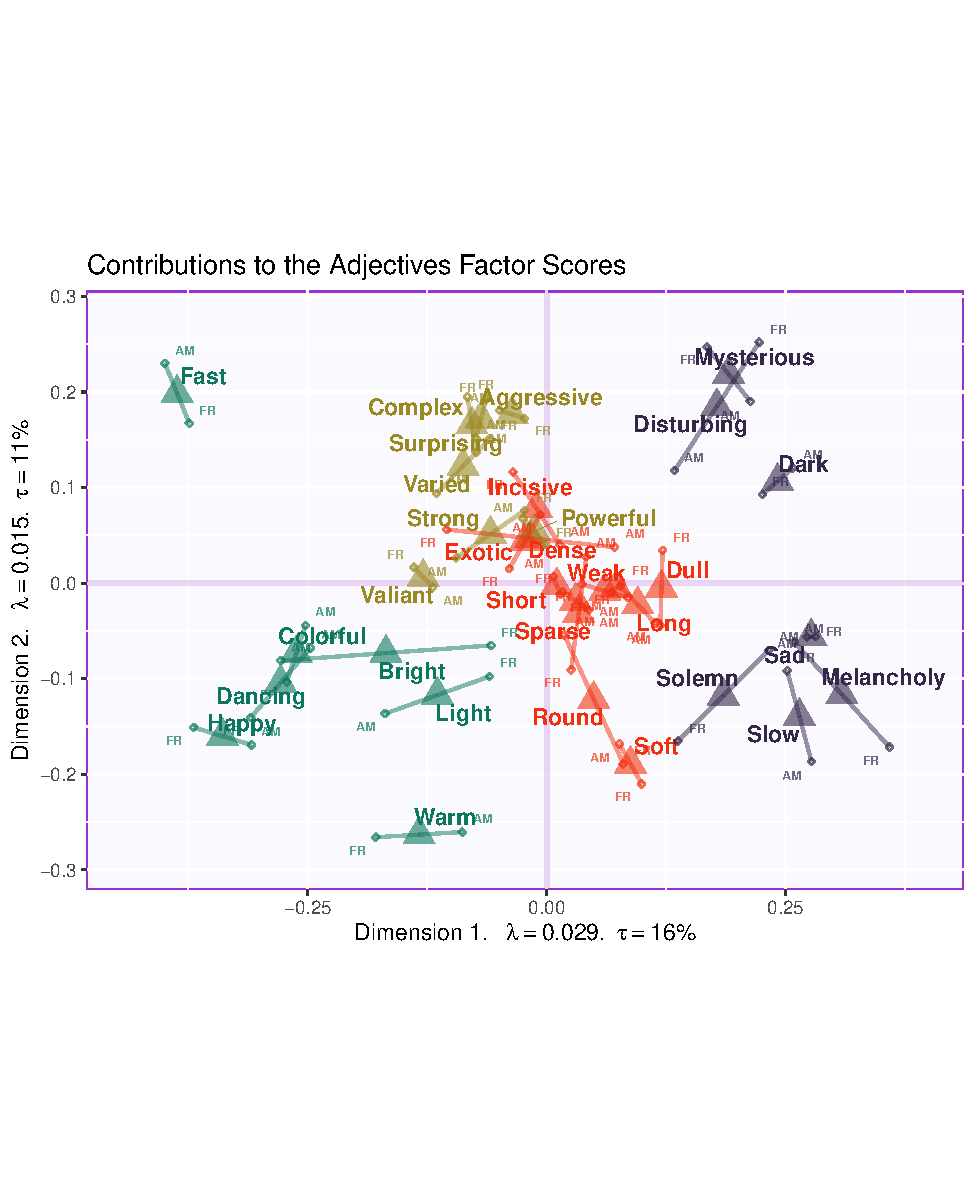
\includegraphics[width=\textwidth]{./Music-Descriptor-Space_files/figure-latex/mfasbs-2}
         %\caption{$y=3sinx$}
         \label{fig:adjectivespfs}
     \end{subfigure}
    \label{fig:mfasbs}
      \caption*{\footnotesize \textit{Note.}  In each plot, the triangles represent the combined factor scores and the small circles represent the partial factor scores contributed by each of the groups.}
\end{figure}

\hypertarget{experiment-3-combined-surveys}{%
\subsection{Experiment 3: Combined Surveys}\label{experiment-3-combined-surveys}}

Experiment 3 used the pseudo-contingency tables from both Experiments 1 and 2, and there was no additional data collected. Since excerpts 6 and 14 were excluded from analysis for Experiment 1, we also removed those rows from the contingency table for Experiment 2. This is so that the dimensions of the two tables for this PLSC would be conformable (remember that we need the same rows or columns in both tables for this analysis). The point of this experiment is to identify the strongest covariance, or the strongest shared signal, between the two tables. Now, this is not to say that these two tables are evaluating the same thing. Instead it allows us to see what is most common between two sets of different information - how often an excerpt was associated with \emph{both} a musical quality and an adjective. The visualizations below allow us to see which variables from each of the two tables correspond with one another; which adjectives are associated with which musical dimensions. Even though both individual tables have their own factor spaces, plotting the common factor space between the two should allow us to see which excerpts are separated from one another using data from both surveys.

\hypertarget{results-1}{%
\subsubsection{Results}\label{results-1}}

\begin{wrapfigure}{h}{.5\textwidth}  
  \begin{center}
    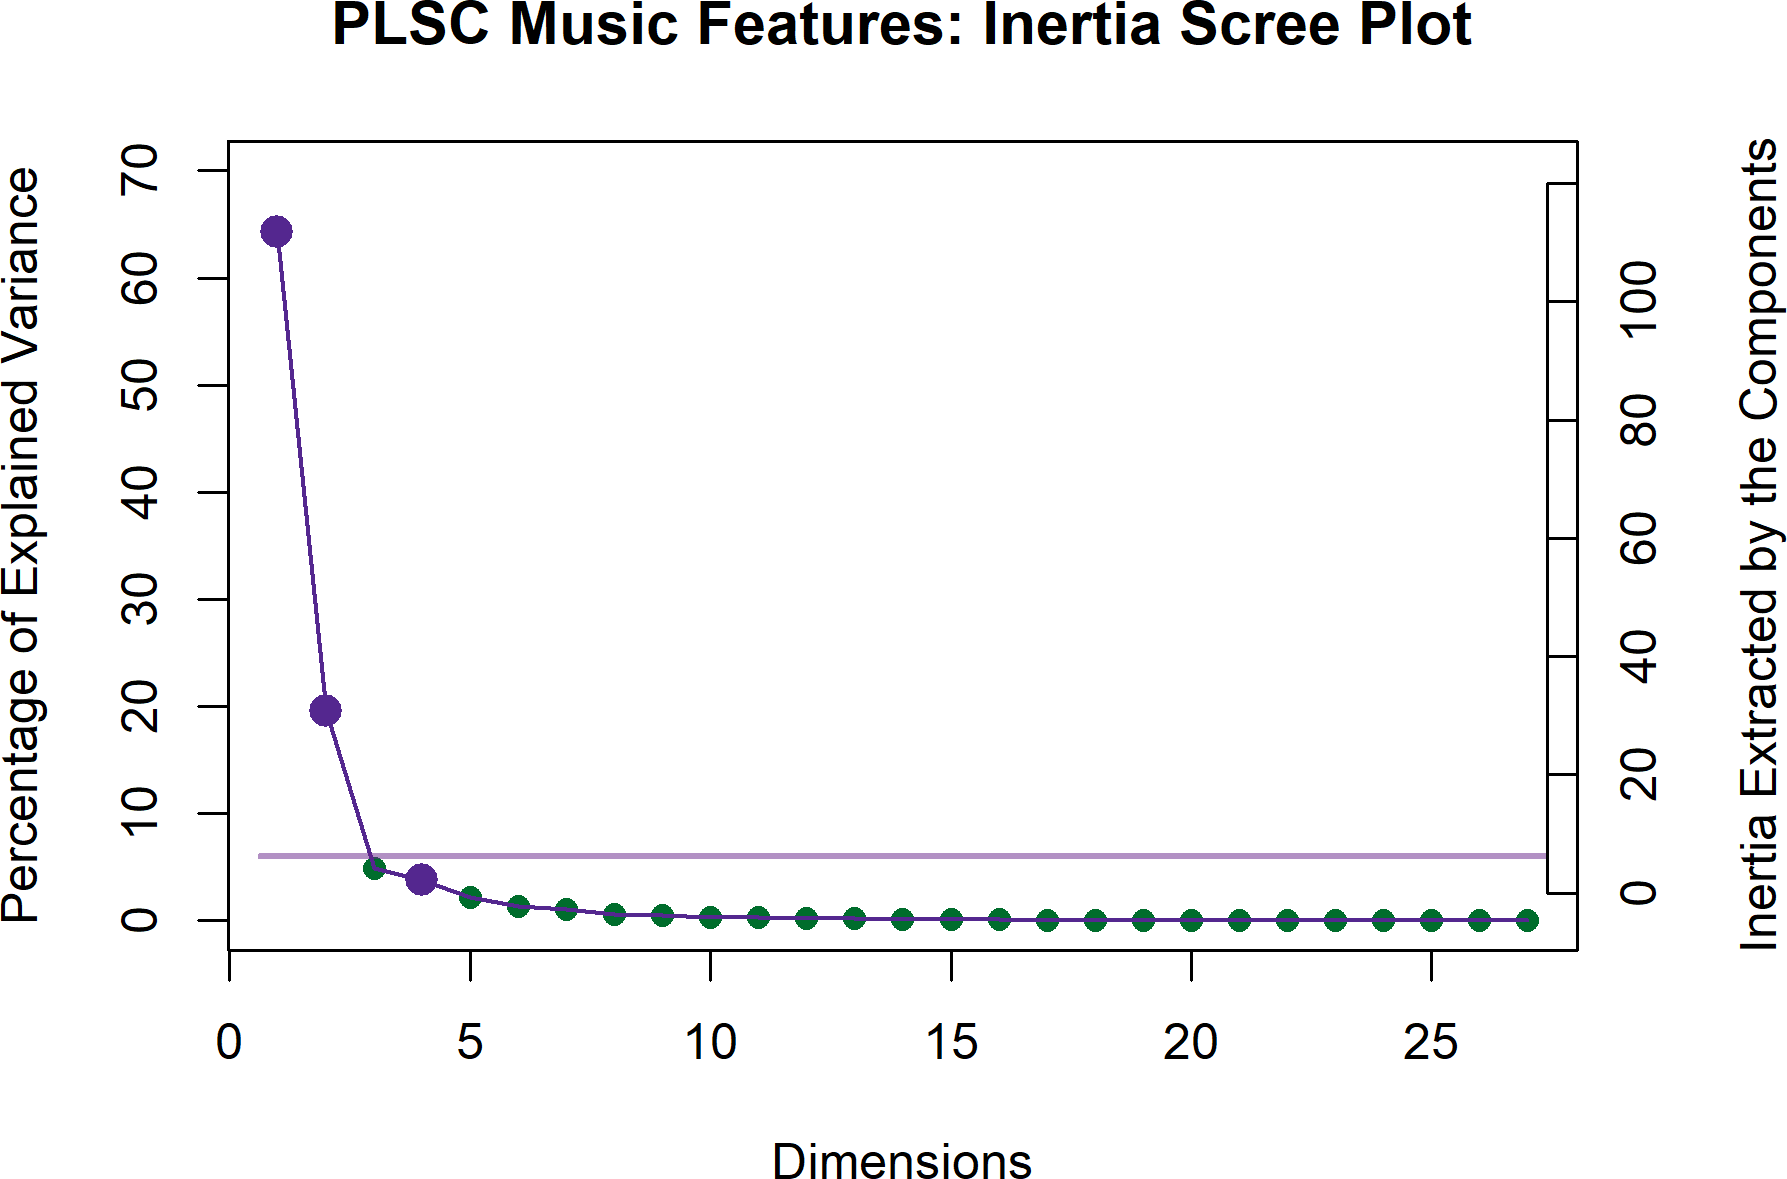
\includegraphics{./Music-Descriptor-Space_files/figure-latex/screePLSC-1.png}
  \caption{ }\label{fig:screePLSC}  
 \end{center}
\end{wrapfigure}

This analysis revealed two dimensions that extracted the majority of the variance (83.60\%). Of that total extracted by the first two dimensions, the first dimension extracted 64.35\% and the second dimension extracted 19.26\%. The scree plot below shows that it's possible that there are two elbows in this graph, at the 3rd and 5th dimensions. The 3rd and 4th dimensions are also significant, extracting 6.02\% and 3.67\% of the variance, respectively. Interpretations of the third dimension and beyond is beyond the scope of this paper, but seeing that there are multiple significant dimensions beyond the second suggests possible future analyses and interpretations using this method.

The plot below shows which variables from each data table load the most on the first and second dimensions. For the purposes of this visualization, we are showing only the variables for which 70\% or more of the variance is explained. The nature of the PLSC also suggests that these are the variables that are most associated with one another between the two tables. The strongest signal on the first dimension juxtaposes the slow and legato musical qualities in the positive direction with the fast, staccato, marcato, and conjunct musical qualities in the negative direction. The adjectives associated with the qualities in the positive direction are ``Dark,'' ``Dull,'' ``Long,'' ``Melancholy,'' ``Sad,'' ``Slow,'' ``Solemn,'' and ``Weak.'' The adjectives associated with the negative direction are ``Bright,'' ``Colorful,'' ``Dancing,'' ``Fast,'' ``Happy,'' and ``Light.''\\
The second dimension identified in the positive direction major harmony and mezzo dynamics, associated with ``Light,'' ``Round,'' ``Soft,'' and ``Warm.'' The negative direction is driven by the impressionist genre being associated with ``Aggressive,'' ``Complex,'' ``Dense,'' ``Disturbing,'' ``Powerful,'' and ``Surprising.''

\begin{figure}

{\centering 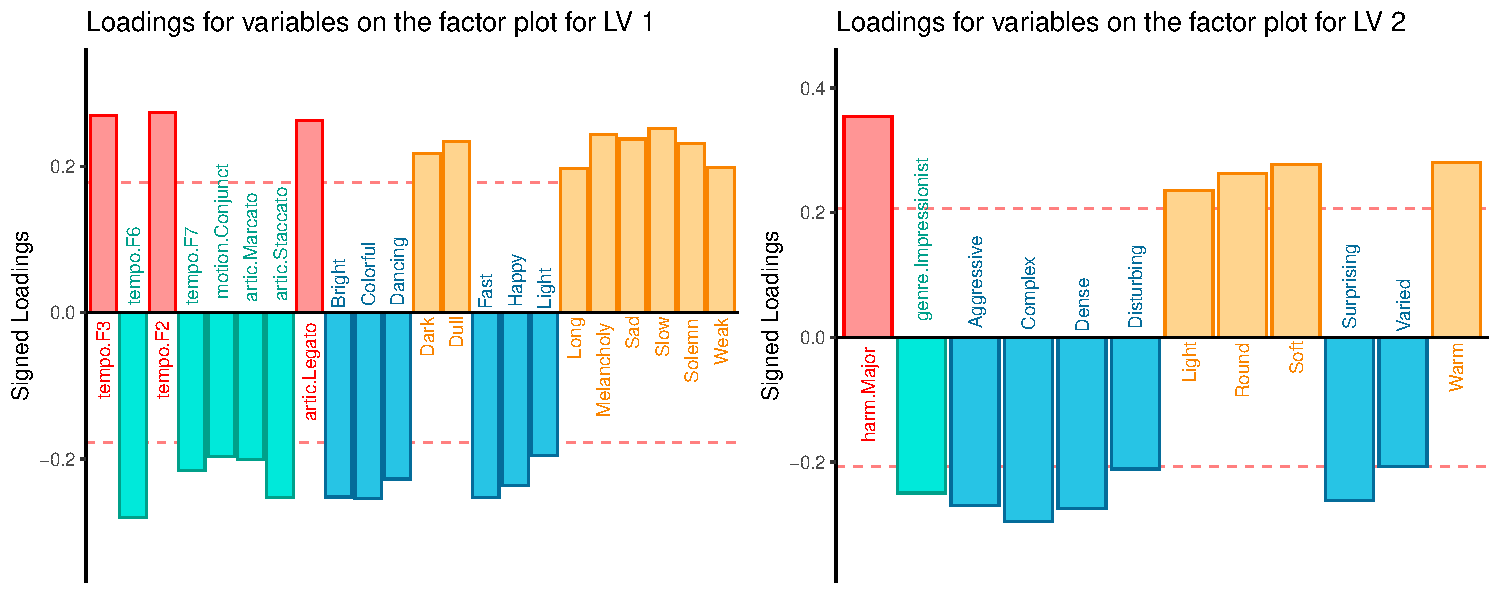
\includegraphics{Music-Descriptor-Space_files/figure-latex/loadingsplsc-1} 

}

\caption{ }\label{fig:loadingsplsc}
\end{figure}

Contributions and loadings are similar, but not exactly the same. A variable's contributions to a dimension are the ratio of the squared factor score to the eigenvalue representing that dimension (Abdi \& Williams, 2010b), and loadings are the correlation between a variable and a component, effectively indicating the shared information between the two. For a more complete disambiguation, see (Abdi \& Williams, 2010b). Figures \ref{fig:contsplsc} and \ref{fig:loadingsplsc} show us that there are quite a few more variables that contribute significantly to these dimensions than for which a significant portion of the variance is explained. We do see similar groups, however: on the first dimension, the tempo variables are contributing significantly, along with some from harmony, density, genre, dynamics, motion, range, and articulation. The adjectives contributing significantly are Bright, colorful, Dancing, Fast, Happy, Light, and Valiant in the negative direction, and Dark, Dull, Long, Melancholy, Monotonous, Sad, Slow, Solemn, and Weak in the positive direction. What's notable here is that while some of these variables did contribute significantly in the plots above (see Figure \ref{fig:factormapsA} and Figure \ref{fig:factormapsQ}), some didn't contribute much at all and fell near the barycenter of the factor plot. We also see that this juxtaposes some negatively and positively valenced adjectives, which allows us to identify which of the musical qualities contributes to the valence dimension.
The second dimension tells us a similar story. Here we see more of the harmony variables, along with one tempo variable, some density, genre, a few dynamics, contour, motion, range, and articulation. The adjectives contributing negatively are Aggressive, Complex, Dense, Disturbing, Incisive, Mysterious, Powerful, Surprising, and Varied, and those contributing positively are Light, Round, Soft, Transparent, and Warm. Again we see similar effects of variables that may not have contributed significantly to their respective plots above, but are contributing significantly here. Also, this second latent variable seems to be defining the arousal dimension.\\

\begin{figure}

{\centering 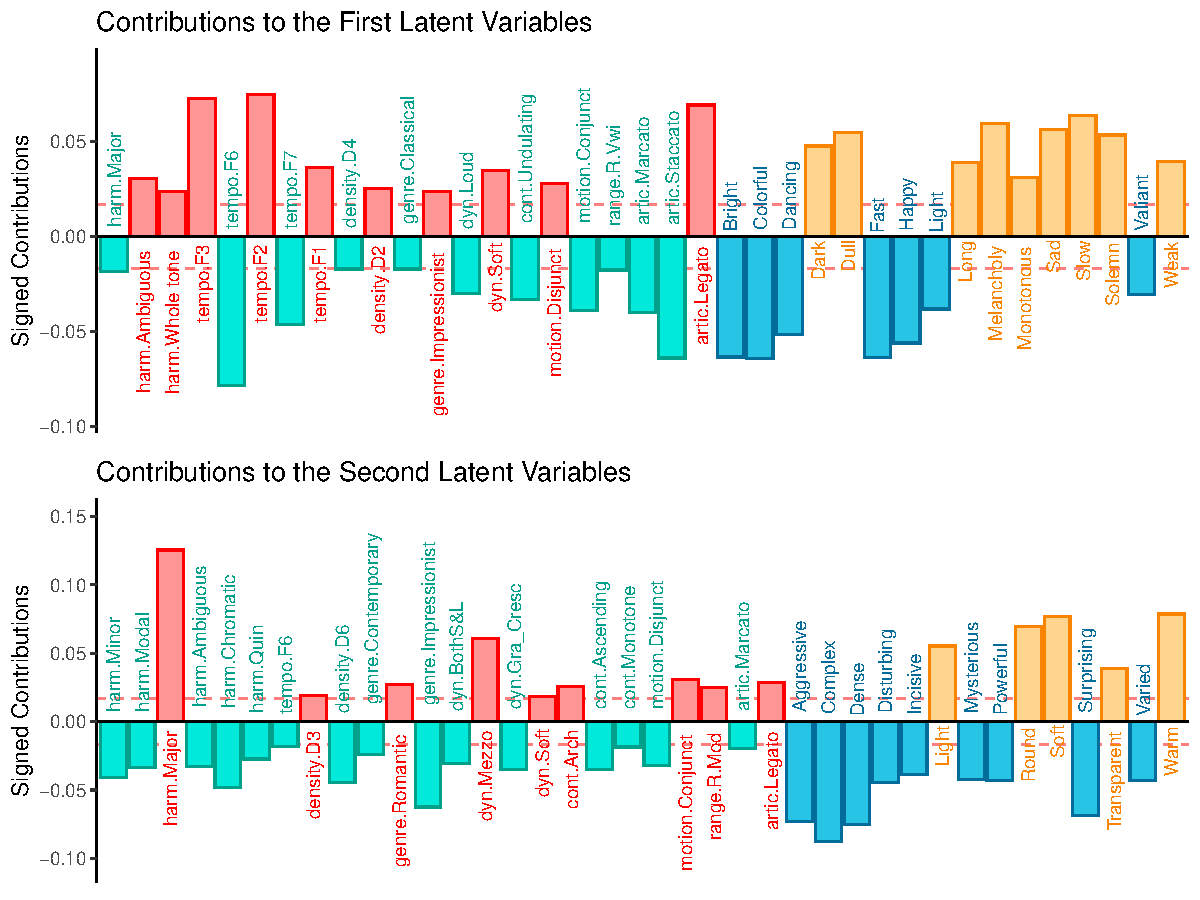
\includegraphics{Music-Descriptor-Space_files/figure-latex/contsplsc-1} 

}

\caption{ }\label{fig:contsplsc}
\end{figure}

\hypertarget{discussion-2}{%
\subsubsection{Discussion}\label{discussion-2}}

The factor score plots for this analysis shows that the first two sets of latent variables extracted by the analysis effectively separate the groups of excerpts into the clusters defined in the HCA for the adjectives survey. This factor plot shows us how the strongest correlated signal between the two data tables separates Excerpts groups 2 and 3, but groups 1 and 2 didn't contribute much to this dimension, instead contributing to the 2nd latent variables. The second latent variable separates Groups 1 and 4, with Groups 2 and 3 more barycentric. This suggests that, generally speaking, the excerpts that were clustered in groups 2 and 3 are those that could be defined by positive and negative valence, respectively, and those in groups 1 and 4 would be defined more by high and low arousal. That being said, these excerpts are not defined exclusively along these dimensions, but rather more by one than the other. For example, Excerpt 26 is characterized by being one of the most extreme examples of positive valence, but doesn't score as highly on the arousal dimension, similarly with Excerpt 27 with negative valence. This is contrasted with Excerpt 7, which is one of the most negatively valenced stimuli, but also scores very high on arousal, although the barycenter for that group is near the origin of that plot.

\begin{figure}

{\centering 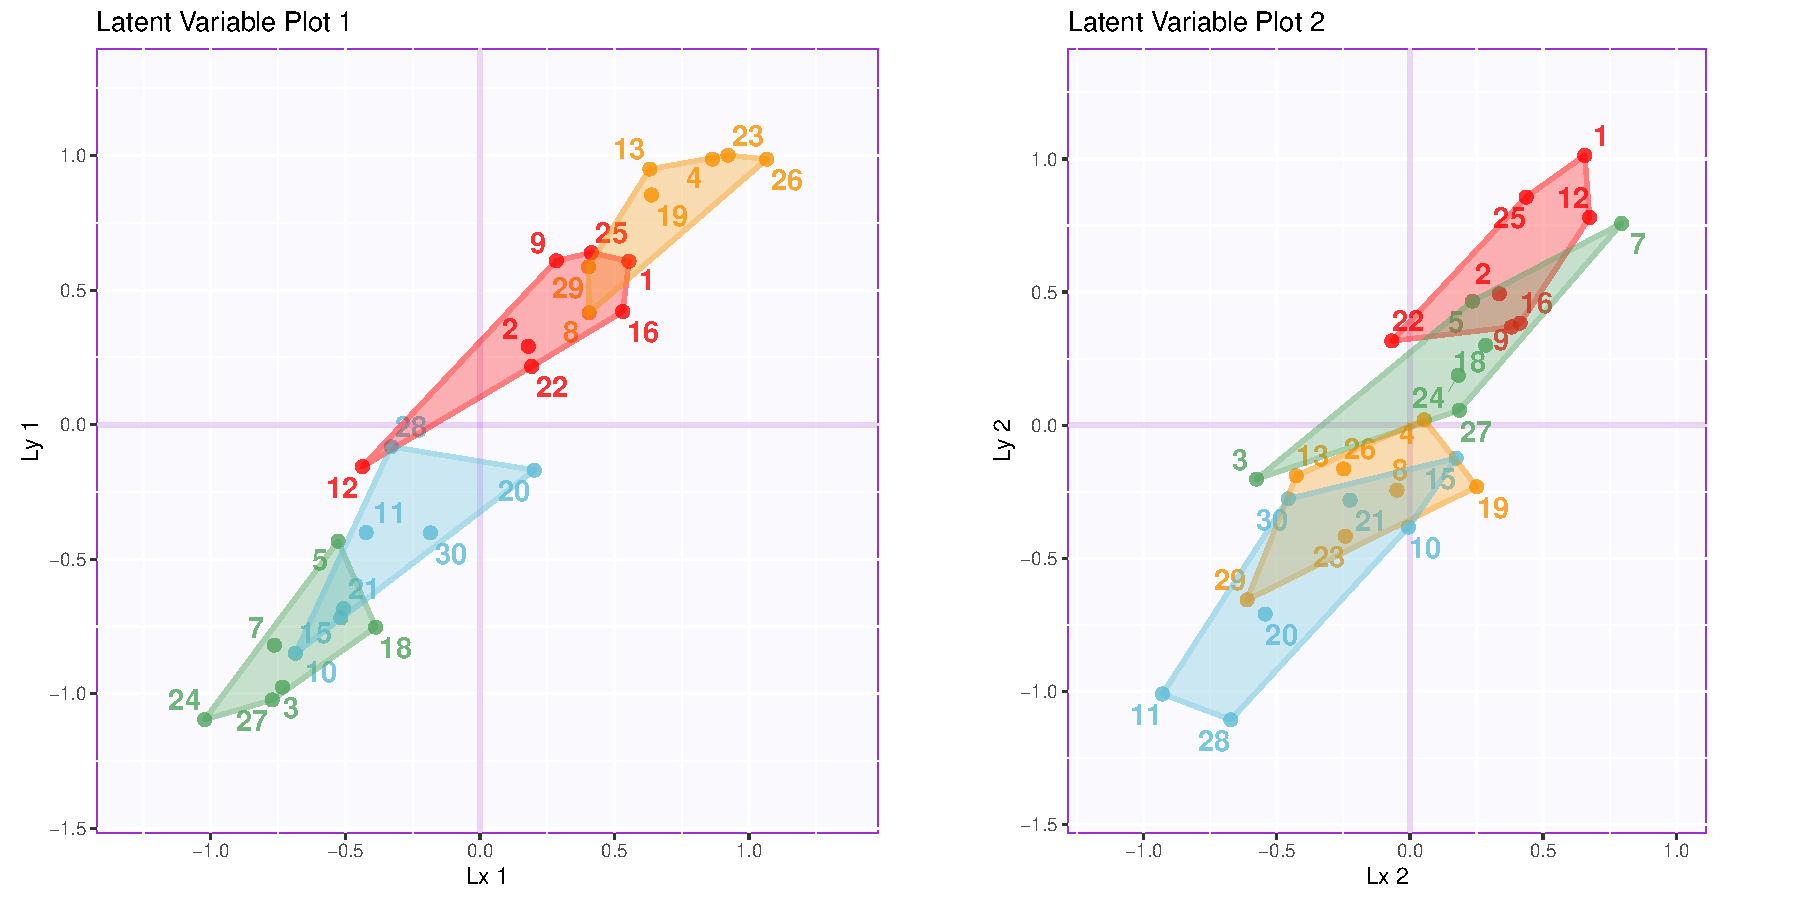
\includegraphics{Music-Descriptor-Space_files/figure-latex/factorplotsPLSC-1} 

}

\caption{ }\label{fig:factorplotsPLSC}
\end{figure}

\hypertarget{general-discussion}{%
\section{General Discussion}\label{general-discussion}}

Although this study was designed to evaluate the sensory or cognitive response to music, and not specifically the emotional response, there is significant overlap in the results observed here and the results of the work investigating music and emotion. The appearance of the valence-arousal plane in the results of Experiment 2 was not unexpected, even though the adjectives we selected were not intended to be explicitly emotional. This goes to show difficult it is to avoid any emotional content when selecting descriptors, and from another perspective, how much emotional contagion the musical examples carry. Overall, this supports the idea that the first two dimensions on which music is judged holistically are valence and arousal.
Some of the results discussed in Experiment 1 require more explanation. In that experiment, there was an issue of having two individual excerpts dominate the factor space, numbers 6 and 14, which did not happen in Experiment 2. One of the differences between CA and PCA is that PCA is distorted by raw values, so bigger numbers have more influence on the overall factor space, but CA finds the average observation. Information that is common, therefore, falls towards the center of the plot, while information that is further from the average, in other words, more rare, ends up further from the center of the factor plots (Abdi \& Williams, 2010a). Therefore, if a survey like the one used in Experiment 1 includes a item that is wildly different than the others in the set, the ratings will be very different, and that item will dominate the factor space. In this case we have two such examples: excerpts 6 and 14. Excerpt 6 was written as a Steve-Reich-esque minimalist, ostinato based excerpt, and excerpt 14 was written to be jazzy. The reason this effect occurs with the first survey and not the second is that the musical qualities on which the excerpts were rated were explicit and designed to separate the excerpts along the various musical dimensions, while the adjectives survey was designed to evaluate the excerpts more generally on holistic qualities. Excerpt 6 still appears as a minor outlier in the visualizations for the second survey, but does not dominate the space the way it does in the results of the first.
What we did to mitigate that is to use those two excerpts as \emph{supplementary projections}, sometimes also referred to as \emph{out of sample observations}. This allows us to evaluate what information is shared by those outliers with the other elements in the dataset without having them dominate the visualization of the factor space. If, when we projected those values into the factor space, they projected onto the origin or very close to it, we would know that those observations shared no information with the other variables. The fact that they are where they are offers support to the idea that the first survey separates the excerpts approximately by genre. Because the `genre' information isn't shared with the other observations, they are being projected onto the space sharing only the information that does not deal with genre, like tempo or range. What this tells us is that musical qualities surveys captured a result that may have characterized by 4-6 factors, each approximating genre and the qualities associated with that genre and the general affective space captured an entirely different set of information about the stimuli and the perception of the stimuli.\\
The hierarchical cluster analyses revealed different groupings in how the stimuli were rated between the two surveys. The PLSC then showed that when including both sets of data, there was a coherent interpretable factor space on which the excerpts were plotted. Another way to look at the results of the two surveys together would be to run a MFA, similar to the one above that plotted the difference between French and American raters on the adjective survey. This would allow us to calculate a common factor space for the two surveys without separating the first and second dimensions of each. We should note that the results of an MFA would provide us with a picture of the data that is fundamentally different from that provided by the PLSC, as it would be a true `common factor space' instead of a space defined by the covariance. The important question here is simply which question is more important. In the case of these experiments, the PLSC more effectively answered our question about what musical information is commonly associated between the technical and affective qualities.\\
An important overall takeaway from this is that with a deep understanding of the stimuli, we may be able to predict the approximate dimensionality of the solution factor space. In the first survey, the solution was that the first two dimensions separated the stimuli along genre or stylistic lines. Because we used only one stimulus from the minimalist and jazz genres, we had a factor space that was distorted by outliers. To have a solution in which we don't see these specific excerpts as outliers, but as coherent members of a factor space, we would need more examples of those styles. This suggests that when creating surveys or designing stimuli, we should keep in mind that we need multiple items per group, or presumed dimension. This is not to say that we will always be able to a priori predict the factor space of the solution. For example, Experiment 2 may also have benefitted from more minimalist or jazz examples. In a system in which the overall structure is obtained by evaluating the stimuli holistically, having a single outlier will necessarily distort the space, either because it is an outlier in sensory terms or because it is the only stimulus against which there is no direct reference. This in a way embodies the issue described in the introduction, in which a single dimension is noisy. The noise, specifically in Experiment 2, comes from the fact that those participants were likely to be less familiar with mimalism and/or jazz than the trained musicians who took the QS, but the reason the results are overall robust to that noise is that the participants were not asked to rate the excerpts on any explicit dimensions or qualities.

\hypertarget{limitations-future-directions}{%
\subsection{Limitations \& future directions}\label{limitations-future-directions}}

Although we evaluate the scores and ratings of participants from different countries, we recognize that the issue of multiculturality is not addressed to a significant degree in this study, because France and the United States are both western countries that share western musical culture. To truly address this question, it would be very interesting to include participants from multiple, contrasting musical cultures, with languages that are more distinct than English and French. This presents new problems, however, as the specific musical qualities included in the surveys may not all apply to or translate well to other musical cultures. One specific example is harmony. The idea of the scale as the basis for both melodic and harmonic material may not be the same across all musical cultures in which scales exist. For example, in western music, the scale represents the notes that are used in a composition to form both melodies and chords, which are the harmonic material, but also specifically infer an order (Cohn et al., 2001). In carn\(\bar{a}\)tic music, the notes that make up the ragas are not used to create chords, and do not imply a specific order (Raman \& Dowling, 2017). Therefore asking participants to identify the harmonic material may not make sense in all situations, and a better question would be to ask what kind of scale or scales are used in a given excerpt.\\
Also, we suggest that data collected in this way hypothetically have a much greater reach, but recognize that the data collected for these experiments represent a convenience sample that is limited to participants that have access to the internet. Additionally, because of the nature of social media, many of the participants in the researchers' social circles are themselves students, and many of the American participants were psychology students. However, these limitations could be easily remedied in future studies.
Another question that fell beyond the scope of this study is the concept of semantic drift between languages. Although illustrated in Figure \ref{fig:mfasbs}, the source of the differences between French and American participants is not entirely clear. We humbly hazard to guess that some of the sources of the difference include aspects of perception that extend beyond the musical. These could be linguistic sources, such as the physical characteristics of the words themselves (Reilly et al., 2012), the cultural associations with the words, or the frequency of use in either language (B. Thompson et al., 2020). Diving more into those questions of linguistics and semantic drift between languages would be a fascinating future study.
Another interesting study would be to repeat this study using adjectives from specific domains or that that avoid explicit emotional or musical content, to see how music maps onto different sensory spaces. For example, `moist,' `slimy,' `dry,' `puckered,' `smooth.' Although some of these adjectives may carry musical weight, in the context of other words that all relate to haptic sensation, it may provide some interesting feedback regarding how the music maps into other sensory domains.
Finally, using these studies may provide pilot work for the way in which people without language react to music, nonverbal autistic people, for example. Whereas this study explicitly uses language as an interlocutor for music perception, it offers insight into ways to better communicate with people who do not have that ability.

\hypertarget{conclusions}{%
\section{Conclusions}\label{conclusions}}

Expanding the collection and analytical paradigms, and thus expanding scientific scope and perspective, has the added benefit of increasing reach. By expanding the ways in which we collect data, we are able to more readily and consistently reach participants who might normally be excluded from everday research paradigms, specifically racially and ethnically diverse populations, poorer populations, those with limited access to transportation, or who have a disability, or are immunocompromised. Developing investigative paradigms that are accessible on mobile platforms and that reduce participant demand while maintaining rigor and integrity will similarly enable us to reach a much greater subset of the population. If we are able to pair this kind of data gathering with appropriate analysis, we can maintain the standards of scientific integrity that we as a community expect from traditional hypothesis testing. The literature to date in the music cognition domain has focused on a fairly small subset of the multivariate analyses available to investigate these questions. As presented here, the number of ways that exist to analyze the data from a single set of experiments is considerable, and the results of each analysis illuminate different parts of the story the data are telling. Not every form of analysis is appropriate in every context, but understanding how, and perhaps more importantly when, to apply a technique or type of analysis is an important to uncovering new perspectives or insights.

\newpage

\hypertarget{references}{%
\section{References}\label{references}}

\begingroup
\setlength{\parindent}{-0.5in}
\setlength{\leftskip}{0.5in}

\hypertarget{refs}{}
\begin{CSLReferences}{1}{0}
\leavevmode\hypertarget{ref-Abdi2010d}{}%
Abdi, H., \& Williams, L. J. (2010a). {Correspondence Analysis}. In N. Salkind (Ed.), \emph{Encyclopedia of research design}. Sage.

\leavevmode\hypertarget{ref-Abdi2010f}{}%
Abdi, H., \& Williams, L. J. (2010b). {Principal component analysis}. \emph{Wiley Interdisciplinary Reviews: Computational Statistics}, \emph{2}, 433--459.

\leavevmode\hypertarget{ref-Abdi2013a}{}%
Abdi, H., \& Williams, L. J. (2013). {Partial Least Squares Methods: Partial Least Squares Correlation and Partial Least Square Regression}. In B. Reisfeld \& A. N. Mayeno (Eds.), \emph{Methods in molecular biology: Computational toxicology volume II} (Vol. 930, pp. 549--579). Springer Science+Business Media, LLC. \url{https://doi.org/10.1007/978-1-62703-059-5}

\leavevmode\hypertarget{ref-Abdi2013}{}%
Abdi, H., Williams, L. J., \& Valentin, D. (2013). {Multiple factor analysis: Principal component analysis for multitable and multiblock data sets}. \emph{Wiley Interdisciplinary Reviews: Computational Statistics}, \emph{5}, 149--179. \url{https://doi.org/10.1002/wics.1246}

\leavevmode\hypertarget{ref-Ares2010}{}%
Ares, G., Deliza, R., Barreiro, C., Giménez, A., \& Gámbaro, A. (2010). {Comparison of two sensory profiling techniques based on consumer perception}. \emph{Food Quality and Preference}, \emph{21}(4), 417--426. \url{https://doi.org/10.1016/j.foodqual.2009.10.006}

\leavevmode\hypertarget{ref-Balkwill2004}{}%
Balkwill, L. L., Thompson, W. F., \& Matsunaga, R. (2004). {Recognition of emotion in Japanese, Western, and Hindustani music by Japanese listeners}. \emph{Japanese Psychological Research}, \emph{46}(4), 337--349. \url{https://doi.org/10.1111/j.1468-5584.2004.00265.x}

\leavevmode\hypertarget{ref-Balkwill1999}{}%
Balkwill, L., \& Thompson, W. F. (1999). {A Cross-Cultural Investigation of the Perception of Emotion in Music : Psychophysical and Cultural Cues}. \emph{Music Perception: An Interdisciplinary Journal}, \emph{17}(1), 43--64. \url{https://doi.org/10.2307/40285811}

\leavevmode\hypertarget{ref-Bartlett1980}{}%
Bartlett, J. C., \& Dowling, W. J. (1980). {Recognition of transposed melodies: A key-distance effect in developmental perspective}. \emph{Journal of Experimental Psychology: Human Perception and Performance}, \emph{6}(3), 501--515. \url{https://doi.org/10.1037/0096-1523.6.3.501}

\leavevmode\hypertarget{ref-Battcock2019}{}%
Battcock, A., \& Schutz, M. (2019). {Acoustically expressing affect}. \emph{Music Perception}, \emph{37}(1), 66--91. \url{https://doi.org/10.1525/MP.2019.37.1.66}

\leavevmode\hypertarget{ref-Benzecri1973}{}%
Benzécri, J.-P. (1973). \emph{{L'analyse des données.}} Dunod.

\leavevmode\hypertarget{ref-Berry2011}{}%
Berry, K. J., Johnston, J. E., \& Mielke, P. W. (2011). {Permutation methods}. \emph{Wiley Interdisciplinary Reviews: Computational Statistics}, \emph{3}(6), 527--542. \url{https://doi.org/10.1002/wics.177}

\leavevmode\hypertarget{ref-Bigand2006}{}%
Bigand, E., \& Poulin-Charronnat, B. (2006). {Are we "experienced listeners"? A review of the musical capacities that do not depend on formal musical training}. \emph{Cognition}, \emph{100}(1), 100--130. \url{https://doi.org/10.1016/j.cognition.2005.11.007}

\leavevmode\hypertarget{ref-Bigand2005}{}%
Bigand, E., Vieillard, S., Madurell, F., Marozeau, J., \& Dacquet, A. (2005). {Multidimensional scaling of emotional responses to music: The effect of musical expertise and of the duration of the excerpts}. \emph{Cognition and Emotion}, \emph{19}(8), 1113--1139. \url{https://doi.org/10.1080/02699930500204250}

\leavevmode\hypertarget{ref-Borg2005}{}%
Borg, I., \& Groenen, P. J. F. (2005). \emph{{Modern Multidimensional Scaling}} (2nd ed., Vol. 36). Springer Science+Business Media, Inc.

\leavevmode\hypertarget{ref-BrunerII1990}{}%
Bruner II, G. C. (1990). {Music, Mood, and Marketing}. \emph{Journal of Marketing}, \emph{October}, 94--104.

\leavevmode\hypertarget{ref-Cohn2001}{}%
Cohn, R., Hyer, B., Dahlhaus, C., Anderson, J., \& Wilson, C. (2001). \emph{{Harmony}}. Oxford University Press.

\leavevmode\hypertarget{ref-Coombs1956}{}%
Coombs, C. H., Milholland, J. E., \& Womer, F. B. (1956). {The assessment of partial knowledge}. \emph{Educational and Psychological Measurement}, \emph{16}(1), 13--37. \url{https://doi.org/10.1177/001316445601600102}

\leavevmode\hypertarget{ref-Cowen2020}{}%
Cowen, A. S., Fang, X., Sauter, D., \& Keltner, D. (2020). {What music makes us feel: At least 13 dimensions organize subjective experiences associated with music across different cultures}. \emph{Proceedings of the National Academy of Sciences of the United States of America}, \emph{117}(4), 1924--1934. \url{https://doi.org/10.1073/pnas.1910704117}

\leavevmode\hypertarget{ref-Darrow1987}{}%
Darrow, A. A., Haack, P., \& Kuribayashi, F. (1987). {Descriptors and Preferences for Eastern and Western Musics by Japanese and American Nonmusic Majors}. \emph{Journal of Research in Music Education}, \emph{35}(4), 237--248. \url{https://doi.org/10.2307/3345076}

\leavevmode\hypertarget{ref-Dowling1978a}{}%
Dowling, W. J. (1978). {Scale and Contour: Two Components of a Theory of Memory for Melodies}. \emph{Psychological Review}, \emph{85}(4), 341--354. \url{https://doi.org/10.1037/0033-295X.85.4.341}

\leavevmode\hypertarget{ref-Drake1999}{}%
Drake, C., Gros, L., \& Penel, A. (1999). {How fast is that music? The relation between physical and perceived tempo.} \emph{Music, Mind, and Science}, \emph{101}, 190--203.

\leavevmode\hypertarget{ref-Escofier-Cordier1965}{}%
Escofier-Cordier, B. (1965). \emph{{L'analyse des correspondances}} {[}Doctoral Thesis{]}. Universit{é} de Rennes.

\leavevmode\hypertarget{ref-Fritz2009}{}%
Fritz, T., Jentschke, S., Gosselin, N., Sammler, D., Peretz, I., Turner, R., Friederici, A. D., \& Koelsch, S. (2009). {Universal Recognition of Three Basic Emotions in Music}. \emph{Current Biology}, \emph{19}(7), 573--576. \url{https://doi.org/10.1016/j.cub.2009.02.058}

\leavevmode\hypertarget{ref-Gray1967}{}%
Gray, P. H., \& Wheeler, G. E. (1967). {The Semantic Differential as an Instrument to Examine the Recent Folksong Movement}. \emph{Journal of Social Psychology}, \emph{72}(2), 241--247. \url{https://doi.org/10.1080/00224545.1967.9922321}

\leavevmode\hypertarget{ref-Greenacre1984}{}%
Greenacre, M. J. (1984). \emph{{Theory and Applications of Correspondence Analysis}}. Academic Press.

\leavevmode\hypertarget{ref-Gregory1996}{}%
Gregory, A. H., \& Varney, N. (1996). {Cross-cultural comparisons in the affective response to music}. \emph{Psychology of Music}, \emph{24}(1), 47--52. \url{https://doi.org/10.1177/0305735696241005}

\leavevmode\hypertarget{ref-Hesterberg2011}{}%
Hesterberg, T. (2011). {Bootstrap}. \emph{Wiley Interdisciplinary Reviews: Computational Statistics}, \emph{3}(6), 497--526. \url{https://doi.org/10.1002/wics.182}

\leavevmode\hypertarget{ref-Juslin2010}{}%
Juslin, P. N., \& Sloboda, J. A. (Eds.). (2010). \emph{{Handbook of music and emotion: Theory, research, applications.}} Oxford University Press.

\leavevmode\hypertarget{ref-Juslin2008a}{}%
Juslin, P. N., \& Västfjäll, D. (2008). {All emotions are not created equal: Reaching beyond the traditional disputes}. \emph{Behavioral and Brain Sciences}, \emph{31}, 559--621. \url{https://doi.org/doi:10.1017/S0140525X08005554\%20Patrik}

\leavevmode\hypertarget{ref-Kamenetsky1997}{}%
Kamenetsky, S. B., Hill, D. S., \& Trehub, S. E. (1997). {Effect of tempo and dynamics on the perception of emotion in music}. \emph{Psychology of Music}, \emph{25}(2), 149--160. \url{https://doi.org/10.1177/0305735697252005}

\leavevmode\hypertarget{ref-Katz1933}{}%
Katz, D., \& Braly, K. (1933). {Racial stereotypes of one hundred college students}. \emph{Journal of Abnormal and Social Psychology}, \emph{28}(3), 280--290. \url{https://doi.org/10.1037/h0074049}

\leavevmode\hypertarget{ref-Kennedy2013}{}%
Kennedy, J., Kennedy, M., \& Rutherford-Johnson, T. (2013). \emph{Harmony} (6th ed.). Oxford University Press.

\leavevmode\hypertarget{ref-Kopacz2005}{}%
Kopacz, M. (2005). {Personality and music preferences: The influence of personality traits on preferences regarding musical elements}. \emph{Journal of Music Therapy}, \emph{42}(3), 216--239. \url{https://doi.org/10.1093/jmt/42.3.216}

\leavevmode\hypertarget{ref-Krishnan2011}{}%
Krishnan, A., Williams, L. J., McIntosh, A. R., \& Abdi, H. (2011). {Partial Least Squares (PLS) methods for neuroimaging: A tutorial and review}. \emph{NeuroImage}, \emph{56}(2), 455--475. \url{https://doi.org/10.1016/j.neuroimage.2010.07.034}

\leavevmode\hypertarget{ref-Ladinig2012}{}%
Ladinig, O., \& Glenn Schellenberg, E. (2012). {Liking unfamiliar music: Effects of felt emotion and individual differences}. \emph{Psychology of Aesthetics, Creativity, and the Arts}, \emph{6}(2), 146--154. \url{https://doi.org/10.1037/a0024671}

\leavevmode\hypertarget{ref-Madsen1997}{}%
Madsen, C. K. (1997). {Emotional Response to Music as Measured by the Two-Dimensional CRDI}. \emph{Journal of Music Therapy}, \emph{34}(3), 187--199. \url{https://doi.org/10.1093/jmt/34.3.187}

\leavevmode\hypertarget{ref-Meyners2014}{}%
Meyners, M., \& Castura, J. (2014). {Check-All-That-Apply Questions}. In \emph{Novel techniques in sensory characterization and consumer profiling} (pp. 271--306). CRC Press/Taylor {\&} Francis. \url{https://doi.org/10.1201/b16853-12}

\leavevmode\hypertarget{ref-Osgood1955}{}%
Osgood, C. E., \& Suci, G. J. (1955). {Factor analysis of meaning}. \emph{Journal of Experimental Psychology}, \emph{50}(5), 325--338. \url{https://doi.org/10.1037/h0043965}

\leavevmode\hypertarget{ref-Raman2016}{}%
Raman, R., \& Dowling, W. J. (2016). {Real-Time Probing of Modulations in South Indian Classical (Carnātic) Music by Indian and Western Musicians}. \emph{Music Perception}, \emph{33}(3), 367--393. \url{https://doi.org/10.1525/MP.2016.33.03.367}

\leavevmode\hypertarget{ref-Raman2017}{}%
Raman, R., \& Dowling, W. J. (2017). {Perception of modulations in south indian classical (carnatic) music by student and teacher musicians: A cross-cultural study}. \emph{Music Perception}, \emph{34}(4), 424--437.

\leavevmode\hypertarget{ref-Reilly2012}{}%
Reilly, J., Westbury, C., Kean, J., \& Peelle, J. E. (2012). {Arbitrary symbolism in natural language revisited: When word forms carry meaning}. \emph{PLoS ONE}, \emph{7}(8). \url{https://doi.org/10.1371/journal.pone.0042286}

\leavevmode\hypertarget{ref-Roda2014}{}%
Rodà, A., Canazza, S., \& De Poli, G. (2014). {Clustering affective qualities of classical music: Beyond the valence-arousal plane}. \emph{IEEE Transactions on Affective Computing}, \emph{5}(4), 364--376. \url{https://doi.org/10.1109/TAFFC.2014.2343222}

\leavevmode\hypertarget{ref-Thompson2020}{}%
Thompson, B., Roberts, S. G., \& Lupyan, G. (2020). {Cultural influences on word meanings revealed through large-scale semantic alignment}. \emph{Nature Human Behaviour}, \emph{4}(10), 1029--1038. \url{https://doi.org/10.1038/s41562-020-0924-8}

\leavevmode\hypertarget{ref-Thompson1994}{}%
Thompson, W. F. (1994). {Sensitivity to combinations of musical parameters: Pitch with duration, and pitch pattern with durational pattern}. \emph{Perception {\&} Psychophysics}, \emph{56}(3), 363--374. \url{https://doi.org/10.3758/BF03209770}

\leavevmode\hypertarget{ref-Tucker1958}{}%
Tucker, L. R. (1958). {An inter-battery method of factor analysis}. \emph{Psychometrika}, \emph{23}(2), 111--136. \url{https://doi.org/10.1007/BF02289009}

\leavevmode\hypertarget{ref-Valentin2012}{}%
Valentin, D., Chollet, S., Lelièvre, M., \& Abdi, H. (2012). {Quick and dirty but still pretty good: a review of new descriptive methods in food science}. \emph{International Journal of Food Science {\&} Technology}, 1--16. \url{https://doi.org/10.1111/j.1365-2621.2012.03022.x}

\leavevmode\hypertarget{ref-Wallmark2019}{}%
Wallmark, Z. (2019). {A corpus analysis of timbre semantics in orchestration treatises}. \emph{Psychology of Music}, \emph{47}(4), 585--605. \url{https://doi.org/10.1177/0305735618768102}

\leavevmode\hypertarget{ref-Wedin1969}{}%
Wedin, L. (1969). {Dimension Analysis of Emotional Expression in Music}. \emph{Swedish Journal of Musicology}, \emph{51}, 119--140.

\leavevmode\hypertarget{ref-Wedin1972}{}%
Wedin, L. (1972). {Evaluation of a Three-Dimensional Model of Emotional Expression in Music}. \emph{The Psychological Laboratories}, \emph{54}(349), 1--17.

\leavevmode\hypertarget{ref-Zacharakis2014}{}%
Zacharakis, A., Pastiadis, K., \& Reiss, J. D. (2014). {An Interlanguage Study of Musical Timbre Semantic Dimensions and Their Acoustic Correlates}. \emph{Music Perception: An Interdisciplinary Journal}, \emph{31}(4), 339--358. \url{https://doi.org/10.1525/MP.2014.31.4.339}

\leavevmode\hypertarget{ref-Zacharakis2015}{}%
Zacharakis, A., Pastiadis, K., \& Reiss, J. D. (2015). {An Interlanguage Unification of Musical Timbre: Bridging Semantic, Perceptual, and Acoustic Dimensions}. \emph{Music Perception: An Interdisciplinary Journal}, \emph{32}(4), 394--412. \url{https://doi.org/10.1525/MP.2015.32.4.394}

\end{CSLReferences}

\endgroup


\end{document}
